\documentclass{book}
\usepackage[spanish,es-nolists,es-tabla, es-nodecimaldot]{babel} % Asegúrate de incluir 'es-nolists' si no quieres que babel altere las listas.


\addto{\captionsspanish}{%
	\renewcommand{\bibname}{Referencias}
}


\usepackage[DIV=14,BCOR=2mm,headinclude=true,footinclude=false]{typearea}
\usepackage{fancyhdr}
\usepackage{subcaption}
\usepackage{multirow}
\usepackage{siunitx}
\fancypagestyle{plain}{
	\fancyhf{}
	\renewcommand{\headrulewidth}{0pt}
	\fancyfoot[C]{\thepage}
}
\pagestyle{fancy}
\fancyhf{}
\fancyfoot[C]{\thepage}

\usepackage{listings}

\usepackage{hhline}
\usepackage{caption}
\captionsetup[figure]{font=small}
\usepackage[table,dvipsnames]{xcolor}
\usepackage{colortbl} % Necesario para \cellcolor
% Paquete para idioma español

% Paquete para personalizar los márgenes
\usepackage[margin=2.5cm]{geometry}
\usepackage{adjustbox}
%Estos dos paquetes son necesarios para escribir cómodamente los
% los documentos en Español, sin necesidad de utilizar secuencias
% de escape como {\'\i} para poner una "í".
\usepackage{titlesec}
\titleformat{\chapter}[display]
{\normalfont\huge\bfseries}{\chaptertitlename\ \thechapter}{20pt}{\Huge}
\titlespacing*{\chapter}{0pt}{0pt}{40pt}
%Para incluir figuras se necesitarán las macros definidas en este paquete
\usepackage{graphicx}

% Para fijar la posición de las imágenes
\usepackage{float}     
\usepackage{xcolor}
\usepackage[table]{xcolor}
%Este paquete permite incluir y resaltar URLs
\usepackage{url}
\usepackage{amsmath, amssymb, bm}
%Este paquete, cuando se usa pdflatex, formatea el documento añadiendo
% enlaces internos entre las referencias y los objetos referenciados
% (por ejemplos, figuras, tablas, referencias de la bibliografía).
\usepackage[unicode=true, pdfusetitle, bookmarks=true, bookmarksnumbered=false, bookmarksopen=false,
breaklinks=true,pdfborder={0 0 1},backref=false,colorlinks=false]{hyperref}

\usepackage{threeparttable}
\usepackage{tabularx}
\usepackage{booktabs}
\newcommand{\ra}[1]{\renewcommand{\arraystretch}{#1}}
% Paquete para personalizar las listas
\usepackage{enumitem} 
\setlist[itemize]{label=-}

%Este paquete puede ser útil si se quieren incluir algunos símbolos
% especiales en las ecuaciones

\usepackage{array}
\usepackage{gensymb}
%Esta definición permite introducir la dirección de los autores
% y mostrarla convenientemente
\newcommand{\address}[1]{\par {\raggedright #1\vspace{1.4em}\noindent\par}}


%Inicio del documento (hasta que se cierre con \end{document}
% Paquete para personalizar los títulos de las secciones
\usepackage{titlesec}
% Paquete para modificar el formato del abstract
\usepackage{abstract}
% Modificar el formato del abstract
\renewcommand{\abstractnamefont}{\normalfont\large\bfseries}
\renewcommand{\abstracttextfont}{\normalfont\normalsize}
\newcolumntype{C}[1]{>{\centering\arraybackslash}p{#1}}
\renewenvironment{abstract}{
\begin{center}
	\bfseries\abstractname\vspace{-\baselineskip}
\end{center}
\list{}{\leftmargin1.5cm \rightmargin\leftmargin}
\item\relax
}{
\endlist
}



% Paquete para ajustar la tabla de contenidos con etoc
\usepackage{etoc}

% Estilo de artículo para cada capítulo
\titleformat{\chapter}[display]{\normalfont\huge\bfseries}{\chaptertitlename\ \thechapter}{20pt}{\Huge}


\makeatletter
\renewenvironment{thebibliography}[1]
{% Utilizamos \section{Referencias} para que aparezca numerado como una sección normal
	\section{Referencias}
	\list{\@biblabel{\@arabic\c@enumiv}}%
	{\settowidth\labelwidth{\@biblabel{#1}}%
		\leftmargin\labelwidth
		\advance\leftmargin\labelsep
		\@openbib@code
		\usecounter{enumiv}%
		\let\p@enumiv\@empty
		\renewcommand\theenumiv{\@arabic\c@enumiv}}%
	\sloppy
	\clubpenalty4000
	\@clubpenalty \clubpenalty
	\widowpenalty4000%
	\sfcode`\.\@m}
{\def\@noitemerr
	{\@latex@warning{Empty `thebibliography' environment}}%
	\endlist}
\makeatother








\begin{document}
	

	
	
	\let\cleardoublepage\clearpage
	% Comenzar numeración de página con el primer artículo en la tabla de contenidos
	
	\frontmatter
	% Tabla de contenidos
	\tableofcontents
	% Ajustar la profundidad de la tabla de contenidos para evitar la numeración incorrecta
	\etocsetnexttocdepth{2}
      
      

	
	\mainmatter
	% Primer artículo
	\titleformat{\chapter}[display]
	{\normalfont\bfseries}{}{0pt}{\LARGE}
	\chapter{Efecto Hall en p-Germanium.}
	\begin{abstract}
	\footnotesize
	\vspace{\baselineskip}
	Este trabajo se lleva a cabo un estudio del efecto Hall en un semiconductor tipo p de germanio mediante una serie de experimentos diseñados para analizar diversas propiedades electrónicas del material. Se midió el voltaje Hall en función de la intensidad de corriente y del campo magnético aplicado, así como a diferentes temperaturas. Los resultados muestran una relación lineal entre el voltaje Hall y la corriente, confirmando las predicciones teóricas. Además, se calculó la movilidad de los portadores y se analizó cómo esta y la densidad de portadores varían con la temperatura y el campo magnético.
	


	\end{abstract}
	\section{Introducción}
	% ***************************************
	
	\vspace{\baselineskip}
	
	El efecto Hall fue descubierto en 1879 por Edwin Herbert Hall mientras era estudiante de doctorado en la Universidad Johns Hopkins. Motivado por una observación de James Clerk Maxwell que predecía que una corriente eléctrica no sería desviada por un campo magnético, Hall diseñó un experimento para poner a prueba esta hipótesis. En su artículo titulado \emph{On a New Action of the Magnet on Electric Currents}, publicado en el American Journal of Mathematics en 1879 \cite{hall}, Hall describe cómo llevó a cabo su experimento utilizando una delgada lámina metálica colocada entre los polos de un electroimán. Al pasar una corriente a través de la lámina y aplicar un campo magnético perpendicular a la corriente, observó la aparición de una diferencia de potencial transversal al flujo de corriente y al campo magnético, fenómeno que luego se conocería como el efecto Hall​.
	
	\vspace{\baselineskip}
	
	Las primeras investigaciones en las que se aplicó aplicó el efecto Hall para el estudio del p-germanio fueron publicadas a mediados del siglo XX \cite{Dunlap1950}\cite{Gallagher1968}, analizándose las características de cristales individuales de germanio de alta resistividad tipo p, incluyendo el efecto Hall, la resistividad y las características de rectificación del material. Las mediciones se realizaron en función de cambios de temperatura y campo magnético, proporcionando datos sobre la movilidad y el coeficiente Hall del germanio tipo p. 
	
	\vspace{\baselineskip}
	
	Estas investigaciones sentaron las bases para desarrollos tecnológicos clave en la electrónica y la instrumentación de sensores, y proporcionaron un marco teórico y experimental sólido para futuras investigaciones en la física del estado sólido. Estos estudios también demostraron la importancia del efecto Hall como una herramienta para caracterizar materiales semiconductores, lo que sigue siendo relevante en la investigación y desarrollo de nuevos materiales y dispositivos electrónicos.
	
    
	
	
	\section{Fundamento teórico}
	% ***************************************
	El efecto Hall se manifiesta cuando un conductor con corriente eléctrica se expone a un campo magnético perpendicular, induciendo un voltaje transversal conocido como voltaje Hall. Este fenómeno se fundamenta en la fuerza de Lorentz, que se define como:
	
	\vspace{\baselineskip}

	\begin{equation} \label{eq:lorentz}
		\mathbf{F} = q(\mathbf{E} + \mathbf{v} \times \mathbf{B})
	\end{equation}
	
	\vspace{\baselineskip}
	
	donde \( q \) es la carga del portador, \( \mathbf{v} \) su velocidad, y \( \mathbf{B} \) el campo magnético.
	
	\vspace{\baselineskip}
	
	En condiciones de equilibrio, la fuerza neta sobre los portadores de carga es nula, lo que establece la relación:
	
	\vspace{\baselineskip}
	
	\begin{equation} \label{eq:equilibrio}
		\mathbf{E} = -\mathbf{v} \times \mathbf{B}
	\end{equation}
	
	\vspace{\baselineskip}
	
	Esta ecuación refleja cómo el campo eléctrico inducido \( E_y \) es directamente proporcional a la velocidad de los portadores y la intensidad del campo magnético, expresado como:
	
	
	\begin{equation} \label{eq:Ey}
		E_y = -v_x B_z
	\end{equation}
	
	 \begin{figure}[H]
	 	\centering
	 	\begin{minipage}{0.55\textwidth} 
	 		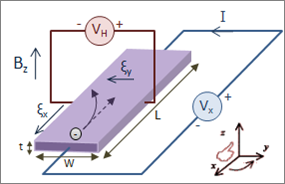
\includegraphics[width=\textwidth]{grafico_1_x00_Hall_Effect_Measurement_Setup_for_Electrons.png}
	 		\caption{Montaje explicativo del efecto hall (Wikipedia).}
	 		\label{fig:efecto_hall}
	 	\end{minipage}
	 \end{figure}
	
	El voltaje Hall, resultante de esta distribución de carga, se calcula por la ecuación:
	
	\vspace{\baselineskip}
	
	\begin{equation} \label{eq:voltaje_hall}
		V_H = E_y w
	\end{equation}
	
	\vspace{\baselineskip}
	
	siendo $w$ el ancho del conductor. Además, la relación entre la velocidad de los portadores y la corriente eléctrica se expresa como:
	
	
	\begin{equation} \label{eq:vx}
		v_x = \frac{I}{n\cdot (-q) \cdot w \cdot t}
	\end{equation}
	
	\vspace{\baselineskip}
	
	donde $I$ es la corriente, $n$ la densidad de portadores de carga, $t$ el espesor de la muestra y $q$ la carga elemental. Sustituyendo [\ref{eq:vx}] y [\ref{eq:Ey}] en [\ref{eq:voltaje_hall}], obtenemos
	
	\vspace{\baselineskip}
	
	\begin{equation} \label{eq:final_VH}
		V_H = \frac{I B_z}{n\cdot q \cdot t}
	\end{equation}
	
	\vspace{\baselineskip}
	
	que proporciona un medio para medir tanto la densidad de portadores como la magnitud del campo magnético.	

	\vspace{\baselineskip}
	
	Por otra parte, de acuerdo a Shockley \cite{Shockley1950}, en este proceso también entran en juego la movilidad de Hall $\mu_H$ de los portadores de carga y la conductividad intrínseca del semiconductor $\sigma_0$. Ambos fenómenos están relacionados mediante la constante Hall $R_H$:
		
	\vspace{\baselineskip}
		
	\begin{equation} \label{eq:mu_H}
		\mu_H = R_H \cdot \sigma_0, \qquad \text{siendo } \qquad R_H = \frac{1}{qn}
	\end{equation}
	
	\vspace{\baselineskip}
	
	Esto permite expresar la constante Hall en términos de $V_H$.
	
	\vspace{\baselineskip}
		
	\begin{equation} \label{eq:RH}
		R_H = \frac{V_{Hall}\cdot d}{B\cdot I}
	\end{equation}
	
	\vspace{\baselineskip}
		
	El coeficiente de Hall $R_H$ proporciona una medida directa del tipo y la concentración de portadores de carga en un material, siendo una de las características principales de los semiconductores.		

	\clearpage
	
	
	Por otro lado, si consideramos B=0, al aplicar una corriente constante a través de un semiconductor, el potencial medido entre dos puntos de acuerdo a la ley de Ohm viene dada por \ref{eq:VIR}.
	
	\begin{equation} \label{eq:VIR}
		V = IR; \qquad R = \frac{\rho L}{A} = \frac{L}{A\sigma} 
	\end{equation}
	
 	siendo $\rho$ la resistividad, $L$ la longitud de la muestra y $A$ su área transversal. Como la conductividad σ es el inverso de la resistividad, se deduce que $V \propto 1/\sigma$ para una corriente y geometría de muestra constantes. 
 	
 	\vspace{\baselineskip}
 	
 	En semiconductores, en la región de conductividad intríseca, la dependencia exponencial de la conductividad con la temperatura viene dada por \ref{eq:sigma}  donde $E_g$ es la energía de la banda prohibida y $k_b$ la constante de Boltzman. se puede investigar mediante análisis del logaritmo del inverso del potencial medido $\ln \frac{1}{V}$ 
 	
 	\begin{equation} \label{eq:sigma}
 		\sigma =  \sigma_{\infty} e^{-\textstyle \frac{E_g}{2k_bT}} \rightarrow 
 	\end{equation}
 
	Por tanto, en las condiciones indicadas, es posible  estudiar la variación de la conductividad en función de la temperatura simplemente midiendo cambios en el potencial eléctrico. 
	
	\section{Montaje experimental}
	
	
	El dispositivo experimental se centra en una muestra de p-Germanio, a través de la cual se puede hacer circular una corriente o aplicar un voltaje controlado. Para medir las características relevantes del efecto Hall, se disponen dos voltímetros: uno mide la caída de tensión en la dirección perpendicular a la corriente, necesario para el cálculo del voltaje Hall; el otro mide la caída de tensión en la dirección de la corriente, proporcionando información sobre la resistencia longitudinal de la muestra.
	
	\vspace{\baselineskip}
	
	Adicionalmente, se integran sensores para el control de las condiciones experimentales. Un sensor de campo magnético se acopla al p-Germanio, permitiendo medir con precisión la intensidad del campo magnético generado por un conjunto de bobinas. Estas bobinas, a través de las cuales se hace circular corriente, son responsables de crear el campo magnético necesario para observar el efecto Hall.
	
	\vspace{\baselineskip}
	
	También se incluye un sensor de temperatura que monitoriza la temperatura de la muestra en tiempo real. La temperatura es un parámetro crítico en el estudio de semiconductores, dado que afecta la movilidad y concentración de portadores de carga en el material. Un dispositivo calefactor, acoplado al semiconductor, permite ajustar la temperatura de la muestra para estudiar su influencia en las mediciones del voltaje Hall y otras propiedades eléctricas.
	
	\vspace{\baselineskip}
	
	Con este montaje, se analizan las relaciones entre varias magnitudes: voltaje Hall en función de la corriente, intensidad del campo magnético y temperatura, así como la diferencia de potencial en la muestra en relación con la intensidad del campo magnético y la temperatura. Este enfoque permite una caracterización detallada del comportamiento del p-Germanio bajo diferentes condiciones experimentales.


	\section{Propagación de errores}
	
	En lo que se refiere a la propagación de errores, las incertidumbres se han obtenido por la expresión general de propagación lineal de errores para una función $f=f(x_1,x_2...x_n)$, donde cada variable $x_i$  es independiente y las incertidumbres en las medidas son $\Delta x_1, \Delta x_2,....\Delta x_n$. En estas condiciones el valor de $\Delta \emph{f}$ viene dado por la ecuación ~\ref{eq:properr}. 
	
	\begin{equation}\label{eq:properr}
		{\Delta f} = \left|\mathbf{\nabla}f\right|\cdot\mathbf{\Delta x} =  \sum_{i=1}^{n}\left|\frac{\partial f}{\partial x_i}\right|\Delta x_i
	\end{equation}
	
	\vspace{\baselineskip}
	
	No obstante con esta aproximación se asume linealidad local en la función, es decir, en la región donde se propaga el error. En casos de no linealidad en la $f$ y/o las incertidumbres involucradas sean de cierta magnitud, expresiones no lineales como potecias o cocientes los resultados pueden ser significativamente erróneos.
	
	\clearpage	
	
	Es por ello  que en el  caso de expresiones no lineales, se ha optado por hacer una propagación de errores basada en el método de Montecarlo \cite{Anderson_montecarlo_1}, generando 1000 muestras de las variables implicadas de acuerdo a una distribución normal centrada en la medida y tomando la incertidumbre como desviación típica.  Para cada muestra se ha calculado el valor de la función correspondiente siendo la estimación final el valor medio de la distribución obtenida y su incertidumbre la desviación típica. Matemáticamente, el proceso se puede resumir como:
	
	\begin{enumerate}
		\item Generar muestras: \((x_{1j}, x_{2j}, \ldots, x_{nj})\) para \(j = 1, 2, \ldots, N\)
		\item Calcular: \(f_j = f(x_{1j}, x_{2j}, \ldots, x_{nj})\)
		\item Analizar: \(\mu_f = \text{media}(f_j)\), \(\sigma_f = \text{desviación estándar}(f_j)\)
	\end{enumerate}
	
	En el caso de los ajuste por regresión lineal se ha seguido un criterio similar, generándose múltiples regresiones determinando los parámetros de la regresión y sus incertidumbres a partir de los valores centrales y las desviaciones típicas obtenidas.
	
	Dado que la energía de 
	
	
	\section{Experimentos y resultados}	
	
	\subsection{Relación Potencial de Hall - Intensidad}	

	En un primer experimento se ha medido la variación del voltaje Hall en función de la intensidad de corriente en una muestra de p-Germanium de espesor $d=1$ mm. Esto se realiza aplicando un campo magnético $B= 250\pm 1 \text{ mT}$ a la muestra  y variando la corriente. De esta manera se puede determinar la constante de proporcionalidad entre el voltaje Hall y la corriente, así como calcular la densidad de portadores de carga en la muestra. Las incertidumbres en las  medidas del potencial y la intensidad han sido respectivamente $\Delta V = 1$ mV y  $\Delta I = 1$ mA.
	
			
	\begin{figure}[H]
		\centering
		\begin{subfigure}[t]{0.48\textwidth}
			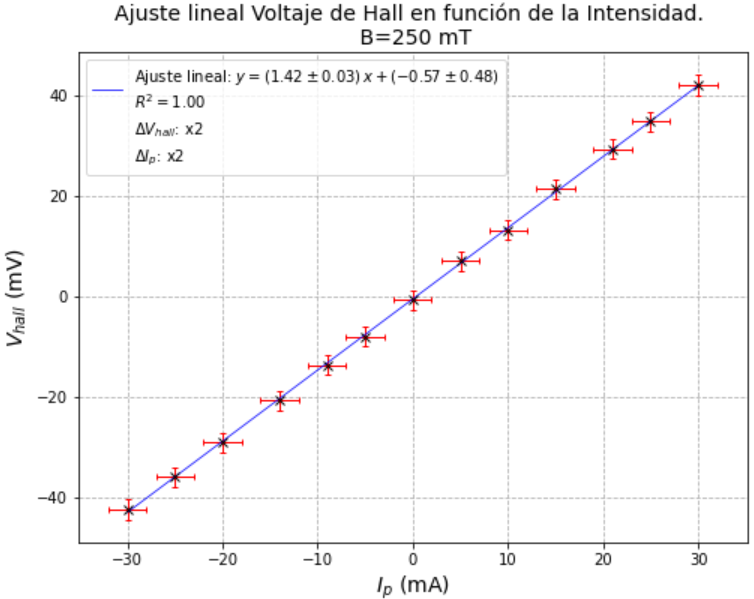
\includegraphics[width=\textwidth]{grafico_1x01_Vhall_vs_Ip.png}
			\caption{}
			\label{fig:Vhall_Ip}
		\end{subfigure}
		\hfill
		\begin{subfigure}[t]{0.48\textwidth}
			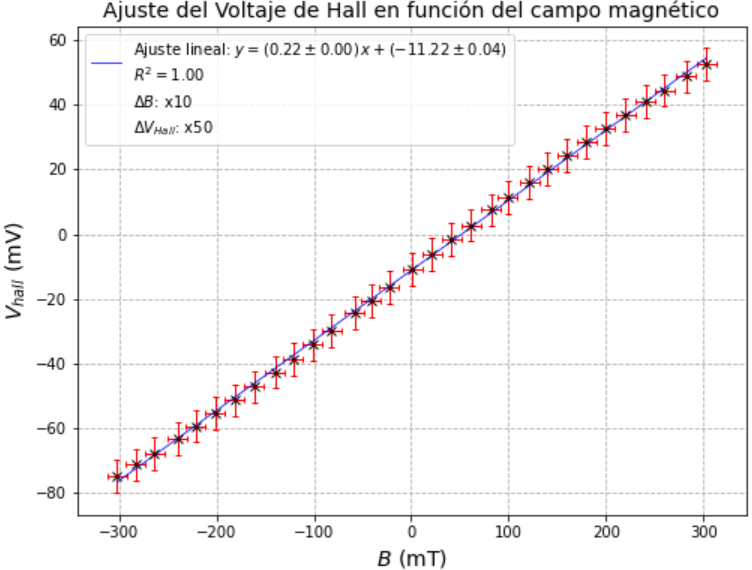
\includegraphics[width=\textwidth]{grafico_1x02_Vhall_vs_B.png}
			\caption{}
			\label{fig:Vhall_B}
		\end{subfigure}
		\caption{\footnotesize{(a) Ajuste lineal de la diferencia de potencial del Hall ($V_{\text{hall}}$), en función de la intensidad de corriente en la placa $I_p$. (b) Ajuste lineal de la diferencia de potencial del Hall ($V_{\text{hall}}$), en función del campo magnético $B$.}}
		\label{fig:hall_plots}
	\end{figure}

	En la figura \ref{fig:Vhall_Ip}, se muestra el resultado del ajuste lineal, $V_{hall}-I_p$ llevado a cabo, donde el resultado obtenido para la pendiente es $\alpha=(1.42\pm 0.03)\Omega$, con coeficiente de determinación R= 1.00, es decir un ajuste lineal exacto en el redondeo al segundo decimal.
	
	\vspace{\baselineskip}
	
	Partiendo por tanto de la relación $V_{Hall} = \alpha I_p$ y teniendo en cuenta \ref{eq:final_VH}, la densidad de portadores n y su incertidumbre mediante propagación lineal se calcula según \ref{eq:denn} y \ref{eq:Denn} respectivamente.
	
	\begin{equation} \label{eq:denn}
		 n = \frac{B}{d\cdot q \cdot \alpha} 
	\end{equation}
	
	
	\begin{equation} \label{eq:Denn}
		\Delta n = \frac{1}{q\cdot d}\left(\left|\frac{1}{\alpha}\right|\Delta B +\left|-\frac{B}{\alpha^2}\right|\Delta \alpha \right)
	\end{equation}
	
	\vspace{\baselineskip}
	
	donde hemos tomado $q$ y $d$ como constantes por lo que $\Delta q =0 $ C y  $\Delta d = 0$ mm. Al hacer los cálculos correspondientes se obtiene una densidad de portadores $n=(1100\pm30)\cdot 10^{18}$ $m^{-3}$.
		

	
	\subsection{Relación Potencial - Intensidad del campo magnético}	
	
	En un segundo experimento se han tomado medias potencial de Hall $V_{Hall}$ y del campo magnético $B$ para una intensidad $Ip=(30\pm1)$ mA. En la figura \ref{fig:Vhall_B}, se muestra el ajuste de los datos donde el valor de la pendiente es b=0.22\pm0.00, con un coeficiente de determinación $R^2=1.00$. 
	
	\vspace{\baselineskip}
	
	Dado que $b=V_{Hall}/B$, podemos calcular el coeficiente de Hall $R_H$ de acuerdo a la expresión \ref{eq:RH},y su error asociado \ref{eq:DRH}.
	
	\begin{equation} \label{eq:DRH}
		\Delta R_H = d\cdot\left(\left|\frac{1}{I}\right|\Delta b +\left|-\frac{b}{I^2}\right|\Delta I \right)
	\end{equation}
	
	\vspace{\baselineskip}
	
	Operando obtenemos $R_H=(7.3\pm0.2)\cdot 10^{-3}$ $m^3/C$. 
	
	\vspace{\baselineskip}
	
	La obtención del valor de $R_H$ permite una via alternativa al cálculo de la densidad de portadores carga n mediante \ref{eq:mu_H}, siendo la incertidumbre en este caso $\Delta n = \left|-\dfrac{1}{q\cdot R_H^2}\Delta R_H\right|$. Operando obtenemos $m^{-3}$.$n=(800\pm20)\cdot 10^{18}$ $m^{-3}$.
	
	\vspace{\baselineskip}
	
	Para determinar la movilidad de los portadores necesitamos previamente el dato de la conductividad inicial a la temperatura que se llevo a cabo el experimento, la cual puede ser calculada a partir de la expresión \ref{eq:VIR}.
	

	\begin{equation} \label{eq:sigma0}
	V_0 = IR_0; \qquad R = \frac{L}{A\cdot\sigma} \rightarrow \boxed{\sigma_0=\frac{I\cdot L}{A\cdot V}} \quad; \qquad \Delta \sigma_0 = \frac{L}{A}\left(\left|
	\frac{1}{V}\right|\Delta I + \left|\frac{-I}{V^2}\right|\Delta V  \right)
	\end{equation} 

	\vspace{\baselineskip}
	
	De acuerdo a los datos tomados en el  experimento 5, el voltaje para la temperatura inicial es de $V=1.69\pm0.01 V$ para una intensidad de corriente $I=30\pm0.001$ mA. Además los valores del area A y la longitud L, tomados como constantes, son $A=10^{-5}$ $m^2$  y $L = 0.02$ m. Operando obtenemos un valor de $\sigma_0 = 36\pm1$ $S\ m^{-1}$ y de aquí obtenemos que $R_0= 56\pm2$ $\Omega$.
	
	\vspace{\baselineskip}
	
	Echo estos cálculos podemos determinar $\mu_H$ \ref{eq:mu_H}, con una incertidumbre $\Delta \mu_H = \sigma_0\Delta R_H + R_H\Delta \sigma_0$. Operando obtenemos el valor $\mu_H = 2630\pm15$ cm$^2$V$^{-1}$s$^{-1}$. De acuerdo a \cite{Madelung2004}, el valor estimado para la movilidad de Hall en huecos para el germanio es   $\mu_h(300 K) = 1800$ cm$^2$V$^{-1}$s$^{-1}$
	
	 
	
	\subsection{Resistencia relativa vs intensidad del campo magnético}	
	
	En este caso se parte de las medidas experimentales de la diferencia de potencial en la muestra $V_s$ para diferentes valores de la intensidad del campo magnético $B$ para una intensidad de polarización $I_p=30\pm1$ mA. Con estos datos es posible determinar los valores de la resistencia $R_m$ para cada voltaje, de manera que la resistencia relativa $R_{rel}$ puede obtenerse según.
	
	\begin{equation} \label{eq:sigma0}
		R_{rel} =  \frac{R_m - R_0}{R_0} =  \frac{V_s/I - R_0}{R_0} = \frac{V_s}{IR}-1
	\end{equation} 

	En este caso la propagación de errores se ha llevado a cabo mediante el método de Montecarlo explicado en la sección 1.4 \cite{error_prop_1}. En la figura \ref{fig:res_rel} se representan los valores de resistencia relativa asociados a cada valor intensidad del campo magnético $B$.
	
	
	\begin{figure}[H]
		\centering
		\begin{minipage}{0.7\textwidth} 
			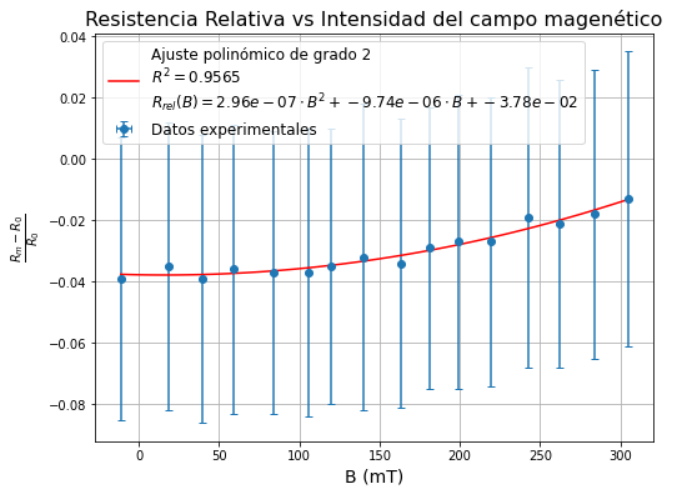
\includegraphics[width=\textwidth]{grafico_1x04_resistencia_relativa_B.png}
			\caption{\footnotesize Ajuste polínomico de grado 2, de la resistencia relativa en función de la intensidad del campo magnético B.}
			\label{fig:res_rel}
		\end{minipage}
	\end{figure}
	
	
	\subsection{Variación del potencial de hall con la temperatura.}
	
	En este experimento se han tomado medidas del potencial de Hall $V_{Hall}$ a diferentes temperaturas para una intensidad de campo magnético $B=300\pm1$ mT y para una intensidad de corriente $I=30\pm1$ mA. En la figura \ref{fig:VH_T}, se muestran estos datos.
 	
	\begin{figure}[H]
		\centering
		\begin{minipage}{0.7\textwidth} 
			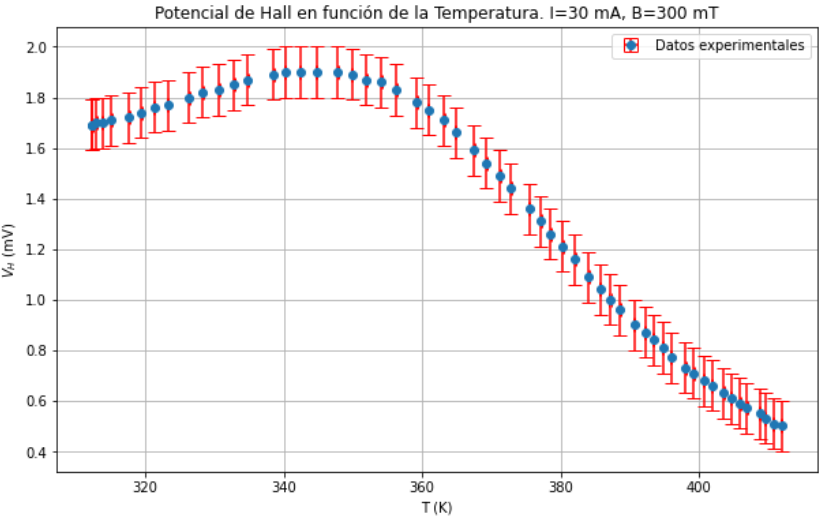
\includegraphics[width=\textwidth]{grafico_1x05_VH_temperatura.png}
			\caption{\footnotesize Representacion de los datos tomados del potencial de Hall en función de la temperatura.}
			\label{fig:VH_T}
		\end{minipage}
	\end{figure}
	
	Se observa que el potencial inicialmente aumenta, alcanzando un máximo de aproximadamente 1.9 mV alrededor de 340 K, para luego disminuir de forma no lineal hasta 0.5 mV a 410 K.
	
	\subsection{Gap de energía en la zona de conductividad intrínseca.}
	
	En este caso dispone se han tomados de datos de la diferencia de potencial en la muestra para diferentes temperaturas para $I=30\pm1 A$ en ausencia de campo magnético B=0. Según lo visto en la introducción teórica, dada la proporcionalidad existente entre 1/V y la conductividad \ref{eq:sigma}. Por tanto al representar  $\ln(1/V)$ s $1/T$ \ref{fig:sigma_intr} , estamos obteniendo un curva proporcional a $\ln(\sigma)$. Esto permite determinar la energía de la banda prohibida $E_g$.
	
	\begin{figure}[H]
		\centering
		\begin{minipage}{0.7\textwidth} 
			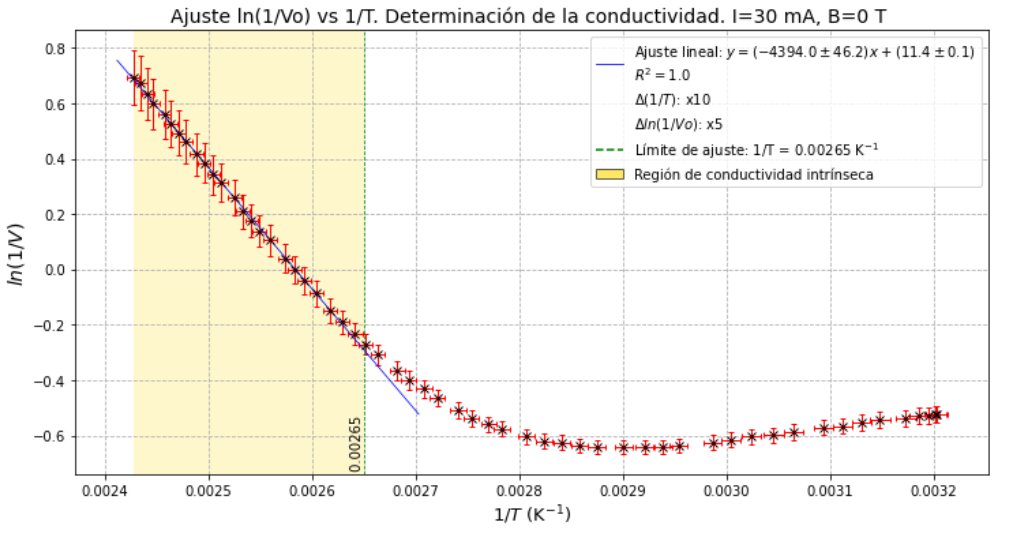
\includegraphics[width=\textwidth]{grafico_1x03_conductividad_intrinseca.png}
			\caption{\footnotesize Gráfico $1/T$ vs $\ln(1/V_0)$. Ajuste lineal en la zona de conductividad intrínseca del semiconductor.}
			\label{fig:sigma_intr}
		\end{minipage}
	\end{figure}
	
	Este curva se obtuvo en el rango 312.2-412 K y exhibe un comportamiento claramente no lineal. No obstante  para valores bajos de  $1/T$ (temperaturas altas), nos situamos en la zona de conducción intrínseca y en ella es posible hacer un ajuste linear \ref{eq:fit_sigma}.
	
	
	\begin{equation} \label{eq:fit_sigma}
		ln(\sigma) = b\cdot \frac{1}{T} + a; \qquad b = -\frac{E_g}{2k_b};\quad a \propto \sigma_{\infty}
	\end{equation}
	
	\vspace{\baselineskip}
	
	donde $k_b = 8.617\cdot 10^{-5}$ eV$K^{-1}$ y $b = 4400.0\pm50$ K. Por tanto $E_g = 2b\cdot k_b$. Operando obtenemos $E_g = 0.76\pm0.1$ eV
	
	\section{Discusión}
	
	En primer lugar hemos examinado la relación entre el voltaje Hall y la intensidad de corriente en una muestra de p-Germanio. El ajuste lineal \ref{fig:Vhall_Ip} indica una relación altamente lineal entre estas variables. Esta linealidad respalda la validez de la ecuación $V_{Hall} = \alpha I_p$ dentro del rango de corrientes estudiado, considerando las incertidumbres asociadas. Utilizando este resultado, se calculó la densidad de portadores de carga obteniéndose un valor $n=(1100\pm30)\cdot 10^{18}$ $m^{-3}$.
	
	\vspace{\baselineskip}
	
	
	Posteriormente hemos obtenido la  relación entre el potencial Hall y la intensidad del campo magnético El ajuste lineal muestra una pendiente $b = 0.22 ± 0.00$, con R² = 1.00, indicando una fuerte relación lineal entre $V_{Hall}$ y $B$. Este resultado permite calcular el coeficiente Hall $R_H = (7.3 \pm 0.2) · 10⁻³ m³C^{-1}$.  El valor de $R_H$ ofrece una vía alternativa para calcular la densidad de portadores, obteniéndose $n=(800\pm20)\cdot 10^{18}$ $m^{-3}$. Este resultado, similar en orden de magnitud al obtenido a partir de $\alpha$, es significativamente mayor del valor de referencia \cite{Madelung2004} de $n=2330 \cdot 10^{18}$ $m^{-3}$ para una temperatura de 300 K. Por otro lado se calculó la conductividad inicial σ₀ = 36 ± 1 S m⁻¹ y la resistencia inicial R₀ = 56 ± 2 Ω. Estos valores permitieron determinar la movilidad de Hall $\mu_H = 2630\pm15$ cm$^2$V$^{-1}$s$^{-1}$. Este valor es superior al valor de referencia para la movilidad de huecos en germanio a 300K ($1800$ cm$^2$V$^{-1}$s$^{-1}$) \cite{Madelung2004}.Si asumimos que la temperatura de la muestra estaba en torno a los 300 K,  el origen mas probable de las discrepancias observadas puede residir en que estos valores de referencia son respecto de muestras puras de p-germanio y siendo compatibles nuestros resultados con que la muestra usada en el experimento este dopada que disminuyan el número de portadores.



	\vspace{\baselineskip}
	
	La gráfica \label{fig:res_rel} muestra la relación entre la resistencia relativa $(R_m - R_0)/R_0$ y la intensidad del campo magnético B. Se observa una tendencia no lineal, con la resistencia relativa aumentando (en valor absoluto) a medida que se incrementa el campo magnético. Los datos se ajustan a un polinomio de grado 2 con $R^2 = 0.9565$, sugiriendo una relación cuadrática. Sin embargo,hay señalar la relevancia de las barras de error en los datos experimentales. Estas incertidumbres, derivan de la propagación de errores en el cálculo de la resistencia relativa A pesar de estas incertidumbres, la tendencia general de aumento en la resistencia relativa con el campo magnético es evidente, aunque la magnitud exacta del efecto a campos altos es menos cierta. Por otro lado se observa que las  variaciones relativas son todas negativas indicativo de que  la resistencia del material disminuye al aplicar un campo magnético. Este fenómeno se conoce como magnetorresistencia negativa y es característico de ciertos tipos de semiconductores, particularmente los semiconductores tipo p, como el germanio dopado con huecos utilizado en este experimento. El aumento de la resistencia con el campo magnético es atribuible a la desviación de las trayectorias de los portadores de carga (en este caso, huecos) por la fuerza de Lorentz, lo que resulta en un aumento efectivo de la longitud del camino que recorren los portadores.

	\vspace{\baselineskip} 

	El fenómeno discutido en el párrafo anterior esta conectado con el funcionamiento de los discos duros mecánicos tradicionales. Los bits se almacenan como pequeñas regiones magnetizadas que generan campos magnéticos débiles. El cabezal de lectura, compuesto por un material magnetorresistivo, pasa sobre estas regiones. El campo magnético de cada bit altera la resistividad del material del cabezal, un efecto similar al observado en el experimento con p-germanio, pero mucho más pronunciado en los materiales utilizados en discos duros reales. La relación cuadrática entre el cambio en la resistividad y el campo magnético ($\Delta R/R_0 \propto B^2$), demostrada en el experimento, es crucial para la alta sensibilidad necesaria en la detección de estos campos magnéticos débiles. Esta sensibilidad permite que pequeños cambios en el campo magnético, correspondientes a diferentes bits, se traduzcan en cambios medibles en la resistividad del cabezal, lo que a su vez se interpreta como los datos almacenados.
	
	\vspace{\baselineskip}
	
	Las mediciones del potencial de Hall en función de la temperatura \ref{fig:VH_T} y el análisis de la conductividad eléctrica sin campo magnético \ref{fig:sigma_intr} proporcionan una visión completa del comportamiento del p-germanio con la temperatura. Al estudiar el efecto Hall, observamos que el potencial inicialmente aumenta hasta aproximadamente 340 K, para luego disminuir no linealmente hasta 410 K. Esta tendencia refleja la transición de un régimen dominado por portadores extrínsecos a uno de conducción intrínseca. La disminución del potencial de Hall a altas temperaturas se corresponde directamente con la región de conductividad intrínseca identificada en el análisis de la conductividad eléctrica. En este último, la gráfica de \ref{fig:sigma_intr} una muestra una clara relación lineal para temperaturas superiores a 377 K $(1/T < 0.00265 K^{-1})$. El ajuste lineal en esta región permite calcular una energía de banda prohibida de aproximadamente 0.76 eV, compatible con cierto nivel de dopaje en la muestra. Esto junto con la reducción del potencial de Hall son manifestaciones complementarias del mismo fenómeno: el aumento en la generación térmica de pares electrón-hueco. En las mediciones de efecto Hall, esto se traduce en una reducción del efecto neto debido al movimiento opuesto de electrones y huecos bajo el campo magnético. 



	\section{Conclusiones}
	
	Los experimentos realizados sobre el efecto Hall en una muestra de p-Germanio han arrojado resultados que validan la teoría fundamental de este fenómeno en materiales semiconductores. La fuerte relación lineal observada entre el voltaje Hall y la intensidad de corriente, así como entre el voltaje Hall y el campo magnético aplicado, confirma la robustez de los principios físicos subyacentes. Sin embargo, las estimaciones de la densidad de portadores, obtenidas por dos métodos independientes, revelaron valores significativamente mayores que los de referencia para germanio puro a 300 K. Esta discrepancia, junto con una movilidad de Hall calculada superior a la esperada, sugiere fuertemente que la muestra estudiada presenta un dopaje específico que altera sus propiedades de transporte.
	
	\vspace{\baselineskip}
	
	La variación del potencial de la muestra con el campo magnético a permitido observa el fenómeno de magnetorrestencia, si bien en las incertidumbres obtenidas en el ajuste la tasa de cambio de la resistencia han sido particularmente relevantes. 
	
	\vspace{\baselineskip}
	
	El análisis de la dependencia de la conductividad con la temperatura ha permitido calcular una energía de banda prohibida de aproximadamente 0.76 eV, proporcionando un dato relevante sobre la estructura electrónica del material. Además, se ha comprobado la transición de un régimen de conducción extrínseca a uno intrínseco con el aumento de la temperatura, evidenciado por cambios significativos tanto en el potencial Hall como en la conductividad eléctrica.
	
	\vspace{\baselineskip}

	En conjunto, estos resultados demuestran la efectividad del efecto Hall como herramienta para la caracterización de semiconductores. Aunque los valores obtenidos difieren de los de referencia para germanio puro, proporcionan información a considerar en las propiedades de transporte en muestras dopadas de p-Germanio.
	
	\vspace{\baselineskip}
	
	
	De cara a experimentos futuros, sería recomendable realizar una caracterización precisa del tipo y nivel de dopaje en la muestra, así como llevar a cabo mediciones a diferentes temperaturas para comprender mejor la transición entre regímenes de conducción.

	
	\section{Referencias}
	
	\begin{thebibliography}{99}
	
	\bibitem{hall}
	Hall E. H.,
	\textit{On a New Action of the Magnet on Electric Currents},
	American Journal of Mathematics, Vol. 2, No. 3, , pp. 287-292, (Sep., 1879)
	\url{https://doi.org/10.2307/2369245}.
	
	
	\bibitem{Dunlap1950}
	W. C. Dunlap,
	\textit{Some Properties of High Resistivity P-Type Germanium},
	Physical Review, vol. 79, no. 2, pp. 286-287, 1950.
	\url{https://doi.org/10.1103/PhysRev.79.286}
	
	\bibitem{Gallagher1968}
	J. W. Gallagher,
	\textit{Transverse Magnetoresistance and Hall Effect in p-Type Germanium},
	Physical Review, vol. 171, no. 3, pp. 987-992, 1968.
	\url{https://doi.org/10.1103/PhysRev.171.987}
	
	\bibitem{Shockley1950}
	Shockley, W. (1950),
	\textit{Electrons and Holes in Semiconductors: With Applications to Transistor Electronics},
	New York: D. Van Nostrand Company, Inc.
	
	\bibitem{Anderson_montecarlo_1} Anderson, G. M., \textit{Error propagation by the Monte Carlo method in geochemical calculations}, Geochimica et Cosmochimica Acta, 40(12), 1533-1538, 1976
	
	\bibitem{error_prop_1} Bevington, Philip R., y D. Keith Robinson. \textit{Data Reduction and Error Analysis for the Physical Sciences}. 3ra ed., McGraw-Hill, 2003.
	
	\bibitem{Madelung2004}
	Madelung, O. (2004). Semiconductors: Data Handbook (3rd ed.). Springer-Verlag Berlin Heidelberg. ISBN: 978-3-540-40488-0
	
	\end{thebibliography}	

		

	
	
	\newpage	

	
% Segundo artículo
\titleformat{\chapter}[display]
{\normalfont\bfseries}{}{0pt}{\LARGE}
\chapter{Difracción de rayos X. Ley de Bragg.}
\begin{abstract}
	\vspace{0.2cm}
	\footnotesize En este trabajo se presenta un análisis de la estructura atómica de cristales utilizando la difracción de rayos X y la Ley de Bragg. Se investigaron muestras de fluoruro de litio (LiF) y bromuro de potasio (KBr) mediante técnicas de radiación de frenado y emisión característica. Esto ha permitido determinar experimentalmente los parámetros de red en ambos cristales así como la distancia interplanar.  Además, se estimó la constante de Planck a través de los parámetros obtenidos en los difractogramas y su relación con la energía máxima de la radiación de frenado. Los resultados corroboran las estructuras cristalinas cúbicas centradas en las caras y proporcionan una validación experimental del uso de rayos X en cristalografía.
	
\end{abstract}
\section{Introducción}
% ***************************************

\vspace{\baselineskip}

La difracción de rayos X y la ley de Bragg son elementos fundamentales en el desarrollo de la cristalografía moderna, proporcionando una base sólida para el estudio de la estructura de la materia a nivel atómico.

\vspace{\baselineskip}

El descubrimiento de los rayos X por Wilhelm Conrad Röntgen en 1895 abrió nuevas vías de investigación en el estudio de la materia. La naturaleza exacta de estos rayos fue objeto de debate científico durante varios años. En 1912, Max von Laue propuso que si los rayos X eran ondas electromagnéticas y los cristales estaban compuestos por átomos ordenados periódicamente, debería ser posible observar la difracción de rayos X en cristales.

\vspace{\baselineskip}

William Henry Bragg y su hijo William Lawrence Bragg, basándose en los experimentos de von Laue, investigaron la difracción de rayos X en cristales. En 1913, formularon lo que actualmente se conoce como la Ley de Bragg, proporcionando una explicación matemática precisa del fenómeno de difracción en estructuras cristalinas. Este descubrimiento les valió el Premio Nobel de Física en 1915. Su trabajo confirmó la naturaleza ondulatoria de los rayos X y estableció las bases para el desarrollo de la cristalografía de rayos X como herramienta para el análisis de la estructura interna de la materia.


\section{Fundamento teórico}
% ***************************************
La difracción de rayos X es una técnica fundamental en la caracterización de la estructura cristalina de los materiales. Este fenómeno ocurre cuando un haz de rayos X incide sobre un material con un ordenamiento atómico periódico, como es el caso de los cristales. Los rayos X, debido a su longitud de onda comparable con las distancias interatómicas, son ideales para estudiar la disposición de los átomos dentro de un cristal.

\vspace{\baselineskip}

En un tubo de rayos X, los electrones son emitidos desde un cátodo calentado, lo que se logra mediante el efecto termoiónico. Estos electrones son acelerados hacia el ánodo, que suele estar hecho de un metal pesado como el cobre, con diferencias de potencial elevada, que puede variar entre 10 y 150 kilovoltios.

\vspace{\baselineskip}

Cuando los electrones acelerados alcanzan el ánodo de cobre, interactúan con los átomos del metal de varias maneras. Una parte de estos electrones es desviada o desacelerada bruscamente al pasar cerca de los núcleos de los átomos de cobre. Esta desaceleración repentina genera un tipo de radiación continua conocida como Bremsstrahlung, o radiación de frenado. Esta radiación tiene un espectro amplio y no es específica de ningún elemento en particular.

\vspace{\baselineskip}

Además, algunos electrones tienen suficiente energía para ionizar los átomos de cobre al expulsar electrones de sus capas internas, generalmente de la capa K. Cuando ocurre esta ionización, se crea una vacante en la capa interna del átomo. Para llenar esta vacante, un electrón de una capa superior cae a la capa inferior, liberando así energía en forma de un fotón de rayos X. Este fotón tiene una energía específica que depende del material del ánodo, y en el caso del cobre, genera las conocidas líneas espectrales $K_{alpha}$ y $K_{\beta}$.

\vspace{\baselineskip}

Cuando una muestra cristalina es irradiada con estos rayos X, los átomos del cristal dispersan esta radiación. Si los rayos X dispersados por diferentes planos atómicos están en fase, es decir, si la diferencia de recorrido entre ellos corresponde a un múltiplo entero de la longitud de onda de los rayos X, se produce interferencia constructiva, generando un pico de intensidad en el difractograma, lo cual ocurre para cierto ángulos de incidencia de los rayos X sobre la muestra. Esto  permite aplicar la ley de Bragg para estudiar su estructura. Esta ley se expresa matemáticamente de acuerdo a la expresión \ref{eq:bragg}


\begin{equation} \label{eq:bragg}
n\lambda = 2d \sin \theta
\end{equation}

\vspace{\baselineskip}


donde $n$ es el orden de difracción (número entero), $\lambda$ es la longitud de onda de los rayos X, $d$ es la distancia entre planos atómicos, y $\theta$ es el ángulo entre el haz incidente y los planos atómicos.  Esta ley establece las condiciones para la interferencia constructiva: la diferencia de camino entre rayos reflejados por planos adyacentes debe ser un múltiplo entero de la longitud de onda, y esta diferencia de camino es $2d sin \theta$, como se deduce de la geometría del sistema \ref{fig:difraccion}.

\begin{figure}[H]
\centering
	\begin{minipage}{0.50\textwidth} 
		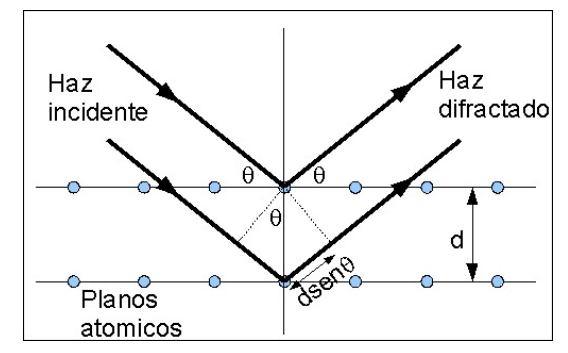
\includegraphics[width=\textwidth]{grafico_2x01_diffraction.png}
		\caption{\footnotesize Geometría de la difracción de rayos X en un cristal.}
		\label{fig:difraccion}
	\end{minipage}
\end{figure}

\vspace{\baselineskip}

Al analizar los patrones de difracción resultantes, es posible determinar la estructura interna del cristal, incluyendo las distancias interplanares y otros parámetros de la red cristalina.


\begin{figure}[H]
	\centering
	\begin{minipage}{0.55\textwidth} 
		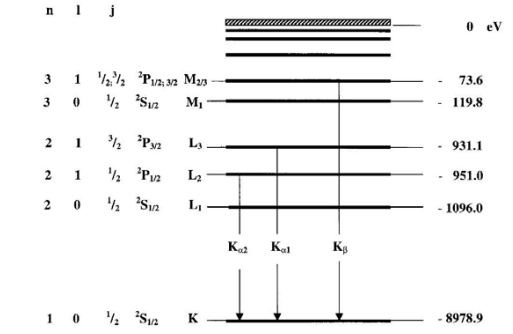
\includegraphics[width=\textwidth]{grafico_2x05_cupper_levels.png}
		\caption{\footnotesize Niveles de energía del cobre (Z=29), tomado de \cite{Haynes2016}}
		\label{fig:culevels}
	\end{minipage}
\end{figure} 



Dado que las energías de las lineas espectrales $K_{\alpha}$ y $K_{\beta}$ son conocidas \ref{fig:culevels} , es posible calcular las longitudes de onda correspondientes de los fotones incidentes $\lambda = hc/\Delta E$ en la muestra, donde $\Delta E$ son los saltos de energía entre la linea original del electrón y la linea $K$ (figura ). Por lo que se puede determinar la distancia entre planos atómicos $d$ a partir de la ley de Bragg de acuerdo \ref{eq:distancia_bragg}.

\vspace{\baselineskip}
\begin{equation} \label{eq:distancia_bragg}
	d = \frac{n\cdot h \cdot c}{2\cdot E\cdot\sin\theta}
\end{equation} 


\vspace{\baselineskip}
La física clásica predice que cuando una partícula cargada, como un electrón, se desacelera en el campo eléctrico de un núcleo, debería emitir radiación electromagnética de manera continua en un espectro, sin un límite superior específico para la energía de los fotones emitidos. Sin embargo, en la realidad, se observa que la radiación de frenado tiene un límite superior en la energía de los fotones emitidos, que corresponde a la energía cinética inicial del electrón antes de su desaceleración.

\vspace{\baselineskip}

Este límite superior se explica adecuadamente por la mecánica cuántica, donde la energía máxima de los fotones de Bremsstrahlung está limitada por la energía cinética del electrón incidente, lo cual es consistente con la conservación de energía en un marco cuántico. Este enfoque cuántico también explica por qué no se pueden emitir fotones con energía mayor que la energía cinética total del electrón desacelerado, algo que la teoría clásica no puede justificar adecuadamente.

\vspace{\baselineskip}

Por lo tanto, la física clásica no puede explicar por qué la radiación de frenado tiene un límite de energía bien definido, lo cual es un claro indicio de la necesidad de un tratamiento cuántico del fenómeno.


\section{Descripción del experimento}


En este experimento, se utiliza la difracción de rayos X para verificar la Ley de Bragg y explorar las estructuras cristalinas de distintos materiales. Se inicia preparando un tubo de rayos X, donde los electrones son emitidos desde un cátodo y acelerados hacia un ánodo, típicamente de cobre, generando rayos X por medio de radiación de frenado y radiación característica.

\vspace{\baselineskip}

Se toman los datos para la creación de  difractogramas para diferentes diferencias de potencial en el LiF y también en el KBr para V=25 kV. Esto proporciona una via para determinar las distancias entre los planos atómicos en la muestra y verificar la estructura cristalina propuesta. Este proceso implica medir los ángulos de difracción y aplicar la ecuación de Bragg para calcular las características estructurales del cristal.

\vspace{\baselineskip}

La muestra cristalina, adecuadamente alineada en el camino de los rayos X, es irradiada, y los patrones de difracción resultantes son observados y medidos. Estos patrones reflejan cómo los rayos X son dispersados por los átomos en la muestra, formando interferencias constructivas en ángulos específicos que satisfacen la Ley de Bragg.


\section{Propagación de errores}

En lo que se refiere a la propagación de errores, las incertidumbres se han obtenido por la expresión general de propagación lineal de errores para una función $f=f(x_1,x_2...x_n)$, donde cada variable $x_i$  es independiente y las incertidumbres en las medidas son $\Delta x_1, \Delta x_2,....\Delta x_n$. En estas condiciones el valor de $\Delta \emph{f}$ viene dado por la ecuación ~\ref{eq:properr_2}. 

\begin{equation}\label{eq:properr_2}
	{\Delta f} = \left|\mathbf{\nabla}f\right|\cdot\mathbf{\Delta x} =  \sum_{i=1}^{n}\left|\frac{\partial f}{\partial x_i}\right|\Delta x_i
\end{equation}

\vspace{\baselineskip}

No obstante con esta aproximación se asume linealidad local en la función, es decir, en la región donde se propaga el error. En casos de no linealidad en la $f$ y/o las incertidumbres involucradas sean de cierta magnitud, expresiones no lineales como potecias o cocientes los resultados pueden ser significativamente erróneos.

\clearpage

Es por ello  que en el  caso de expresiones no lineales, se ha optado por hacer una propagación de errores basada en el método de Montecarlo \cite{Anderson_montecarlo_1}, generando 1000 muestras de las variables implicadas de acuerdo a una distribución normal centrada en la medida y tomando la incertidumbre como desviación típica.  Para cada muestra se ha calculado el valor de la función correspondiente siendo la estimación final el valor medio de la distribución obtenida y su incertidumbre la desviación típica. Matemáticamente, el proceso se puede resumir como:

\begin{enumerate}
	\item Generar muestras: \((x_{1j}, x_{2j}, \ldots, x_{nj})\) para \(j = 1, 2, \ldots, N\)
	\item Calcular: \(f_j = f(x_{1j}, x_{2j}, \ldots, x_{nj})\)
	\item Analizar: \(\mu_f = \text{media}(f_j)\), \(\sigma_f = \text{desviación estándar}(f_j)\)
\end{enumerate}

En el caso de los ajuste por regresión lineal se ha seguido un proceso similar generando múltiples regresiones determinando los parámetros de la regresión y sus incertidumbres a partir de los valores centrales y las desviaciones típicas obtenidas.



\section{Resultados}

\subsection{Estructura cristalina del LiF. Difractogramas}


En esta sección, se presentan los resultados obtenidos de los difractogramas para el fluoruro de litio (LiF) al variar la diferencia de potencial aplicada. La figura \ref{fig:difractogramas_LiF} muestra estos difractogramas, en los cuales se observa que al aumentar el angulo progresivamente desde cero aparece en primera instancia un región donde la intensidad aumenta lentamente sin picos abruptos, donde predomina la dispersión de la radiación frenado. Posteriormente llegamos a una región donde aparecen  dos picos de intensidad, primero uno de menor intensidad y luego uno de mayor intensidad, que corresponden respectivamente a las transiciones electrónicas $K_{\beta}$ y $K_{\alpha}$. La diferente intensidad se debe a que las probabilidades de que ocurran las transiciones electrónicas no son iguales.

\begin{figure}[H]
	\centering
	\begin{minipage}{0.9\textwidth} 
		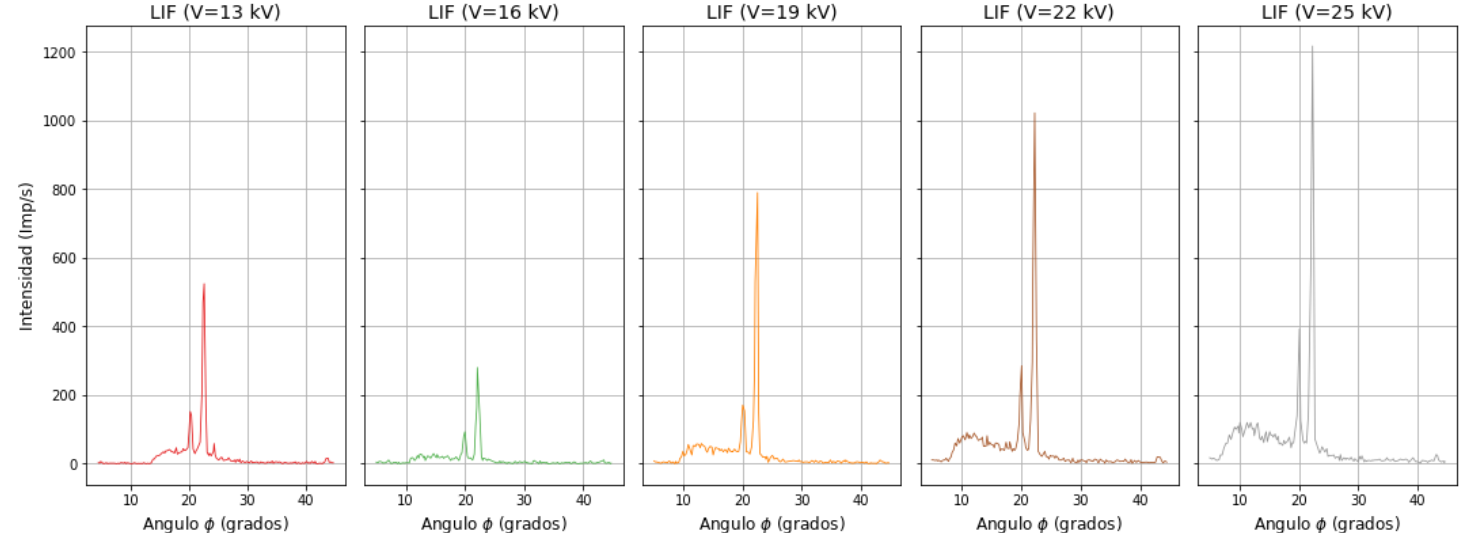
\includegraphics[width=\textwidth]{grafico_2x02_difractogramas_LiF.png}
		\caption{\footnotesize Difractograma de una muestra del fluoruro de litio (LiF) para diferentes diferencias de potencial.  $K_{\beta}$ menos inteso y $K_{\alpha}$ más intenso}.
		\label{fig:difractogramas_LiF}
	\end{minipage}
\end{figure}


El fluoruro de litio (LiF) tiene una estructura cristalina cúbica centrada en las caras (FCC, FaceCentered Cubic) \ref{fig:str_lif}. En esta estructura, los iones de litio ( $\mathrm{Li}^{+}$) y flúor ( $\mathrm{F}^{-}$) están dispuestos en los vértices y en los centros de las caras de la celda unitaria cúbica. Esta disposición es típica de los compuestos iónicos simples y es análoga por ejemplo a la estructura del cloruro de sodio $(\mathrm{NaCl})$ o del bromuro de potasio $KBr$.


\begin{figure}[H]
	\centering
	\begin{minipage}{0.5\textwidth} 
		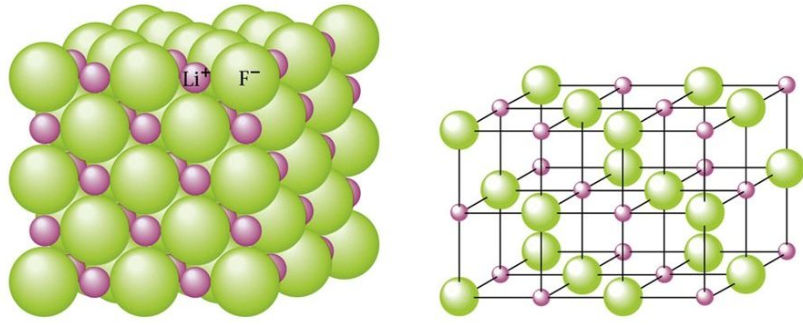
\includegraphics[width=\textwidth]{grafico_2x06_lif_structure.png}
		\caption{\footnotesize Estructura del  fluoruro de litio. Fuente:\cite{strlif}.}
		\label{fig:str_lif}
	\end{minipage}
\end{figure}




\vspace{\baselineskip}

En el caso de una red con estructura cúbica centrada en las caras, el parámetro de red se puede determinar teóricamente a partir de la densidad, la masa molar y la constante de Avogadro. De acuerdo a al bibliografía \cite{LiF_quim}, la densidad del LiF es $\rho = 2.635$ g$\cdot$cm$^{-3}$ y tiene una masa molar  $M=26.01440660$ g$\cdot$ mol$^{-1}$ siendo el número de Avogadro $N_A= 6.02214076\cdot 10^{-23}$ mol$^{-1}$. De acuerdo a \cite{Wahab2021} el parámetro de red viene dada por \ref{eq:param_red}. 

\begin{equation}\label{eq:param_red}
	a=\left(\frac{n \cdot M}{\rho \cdot N_A}\right)^{1 / 3}
\end{equation}



donde $n=4$, que es el número de fórmulas unitarias de LiF en una celda unitaria. Una fórmula unitaria es la unidad más simple de una sustancia química que representa la proporción de elementos en el compuesto. En un cristal, una fórmula unitaria corresponde a la cantidad de cada tipo de átomo o ion que refleja la proporción estequiométrica en la estructura cristalina.

\vspace{\baselineskip}
Después de operar con \ref{eq:param_red}, se obtiene un valor $a_t=4.032$ \AA. Este valor teorico, es una buena aproximación al valor encontrado en la bibliografía \cite{LiF_str}  $a_b=4.028\pm 0.002$ \AA.


\vspace{\baselineskip}


Además, tal y como se explicó en la introducción teórica, a partir de los difractogramas obtenidos se puede calcular\ref{eq:distancia_bragg} la distancia entre los planos cristalinos responsables de la difracción de los rayos X. Esto permitirá hacer una estimación experimental del parámetro de red.

\vspace{\baselineskip}

En el caso del cristal de LiF, hay dos picos que corresponden a las transiciones $\alpha$ $KL_3$ ($K_{\alpha_1}) $ y  $KL_2$ ($K_{\alpha_2})$  con energías respectivas de 8047.78 eV y 8027.83 eV respectivamente \cite{Bearden1967}. Como se ve, ambos saltos energéticos son muy parecidos no teniendo los difractograms llevados a cabo la resolución suficiente  para que puedan distinguirse de forma separada. En este caso, se tomará el valor medio $K_{\bar\alpha}$ \ref{eq:alfa_mean}.

\begin{equation}\label{eq:alfa_mean}
	K_{\bar\alpha} = \frac{1}{2}\left(K_{\alpha_1} + K_{\alpha_2}\right) = 8037.55 \text{ eV} 
\end{equation}

El otro pico adicional corresponde a la  transición $\beta_{1,3}$ entre los niveles $K M_{2,3}$ de 8905.29 eV \cite{Bearden1967}. 

\vspace{\baselineskip}

Con estos datos es posible hacer una estimación de la longitud de onda correspondiente a las transiciones $K_{\bar\alpha}$ y  $K_{\beta}$ aplicando simplemente $\lambda = \frac{hc}{ E}$. Operando se obtiene $\lambda_{\bar\alpha} = 1.54$ \AA y $\lambda_{\beta} = 1.39$ \AA. Con estos valores aplicamos  \ref{eq:bragg} para los ángulos en los que se producen los picos en cada difractograma  (Tabla \ref{tab:d_alfa_beta}).  Para el calculo de $d$ se ha aplicado una propagación lineal de errores siendo $\Delta d_{\bar{\alpha}} = \frac{n\lambda}{2}\left|-\frac{\cos\theta}{\sin^2\theta}\right|\Delta\theta$. 




\begin{table}[H]
	\centering
	$\Delta \theta = \pm0.1^\circ$ = \pm 0.002 rad; \quad Orden difracción: n=1\\
	\begin{tabular}{C{1.5cm} | C{1.5cm} C{2cm} | C{1.5cm} C{2cm}}
		\toprule
		\toprule
		& \multicolumn{2}{c|}{$K_{\alpha}$} & \multicolumn{2}{c}{$K_{\beta}$}  \\
		\cline{1-5}
		V (kV) & $\theta$ ($^\circ$) & $d_{\alpha}$ (\AA)  & $\theta$ ($^\circ$) & $d_{\beta}$ (\AA)    \\
		\hline 
		13 & 20.2 & 2.234$\pm$0.011 & 22.6 & 1.811$\pm$0.008 \\
		16 & 20.0 & 2.255$\pm$0.011 & 22.1 & 1.850$\pm$0.008 \\
		19 & 20.0 & 2.255$\pm$0.011 & 22.5 & 1.819$\pm$0.008 \\
		22 & 20.1 & 2.244$\pm$0.011 & 22.3 & 1.835$\pm$0.008 \\
		25 & 20.1 & 2.244$\pm$0.011 & 22.3 & 1.835$\pm$0.008 \\
		\hline
		\hline 
		\textbf{Media} & & \textbf{2.246$\pm$0.011} & & \textbf{1.830$\pm$0.008} \\
		\bottomrule
		\bottomrule
	\end{tabular}
	\caption{\footnotesize Determinación de la distancia entre planos atómicos en el fluoruro de litio.}
	\label{tab:d_alfa_beta}
\end{table}


El valor medio final es la media de los valores $\bar{d}_{\bar{\alpha}}$ y $\bar{d}_{\beta}$: $d=2.038\pm0.010$ \AA.


\vspace{\baselineskip}


Con el valor $d$ calculado y con el valor teórico del parámetro de red ($a_t$) calculado anteriormente, es posible determinar los índices de Miller.Esto se debe a que en un sistema cúbico se cumple \ref{eq:miller} 

\vspace{\baselineskip}

\begin{equation}\label{eq:miller} 
	d^2_{hkl} = \frac{a^2}{h^2 + k^2 + l^2} \rightarrow \sqrt{h^2 + k^2 + l^2} = \frac{a}{d_{hkl}}
\end{equation} 

\vspace{\baselineskip}

En nuestro caso tenemos que $a_t/d = 4.032/2.038 = 1.98 \approx 2 $. Dado que el LiF tiene simetría cubica centrada en las caras los índices de Miller posibles de acuerdo a la bibliografía  \cite{Cullity2014} son \{200\}. Conocido el plano de difracción es posible hacer una nueva estimación del parámetro de red: $ a_d = 2d = 4.078\pm0.020$ \AA, lo que supone una desviación por exceso entre el 0.8\% y el 1.7\% respecto del valor recogido en la bibliografía.

\vspace{\baselineskip}

La determinación de la distancia $d$ entre planos atómicos nos deja en posición de hacer una estimación de la constante de Planck. Esto se debe a que el borde inferior del espectro de la radiación de frenado determina una energía máxima de la radiación de rayos X, la cual cambia en función de la diferencia de potencial aplicada ($E=e\cdot V$) en el dispositivo generador. Esta relación de la energía con la diferencia de potencial junto con la expresión \ref{eq:distancia_bragg}  permite llegar a la expresión \ref{sinmin}.


\begin{equation} \label{sinmin}
	\sin\theta_{min} = \frac{h \cdot c}{2\cdot d\cdot e}\cdot \frac{1}{V_{min}} \rightarrow h= \frac{2\cdot d\cdot e}{ c}\cdot\gamma
\end{equation} 


En la tabla \ref{tab:sinV} se muestran el ángulo mínimo y el voltaje correspondiente recogidos de los difractogramas \ref{fig:difractogramas_LiF}. Con estos datos se ha verificado \ref{sinmin}, mediante el ajuste de regresión correspondiente que se muestra en la figura \ref{fig:Lif_sin_1_V}. Con el valor de la pendiente de recta regresión ajustada $\gamma = (3046\pm 473)$ V, el valor de la constante de planck de terminado es de $6.63575\pm 1.06291)\cdot 10^{-34}$ J/s, donde se ha aplicado propagación lineal de errores \ref{eq:properr_2}. Como se observa la el valor central es bastante aproximado al valor de referencia de $6.626070\cdot 10^{-34}$ J/s. No obstante la incertidumbre de la estimación realizada llega al 16\%, principalmente por resolución en la medida de los ángulos y por la escasez de puntos obtenidos para hacer el ajuste.

\vspace{\baselineskip}





\begin{table}[H]
	\centering
	\begin{minipage}{0.7\textwidth} 
		\centering
		\footnotesize $\Delta \theta = \pm0.1^\circ = \pm 0.002$ rad; $\Delta V = 1$ kV \\
		\begin{tabular}{|C{1.5cm}|C{1.5cm}|C{1.5cm}|C{1.5cm}|C{1.5cm}|C{1.5cm}|}
			\toprule
			\toprule
			V (kV) & 13 & 16 & 19 & 22 & 25 \\
			\hline
			$\theta_{min}$ ($^\circ$) & 13.8 & 10.8 & 9.4 & 8.4 & 6.8 \\
			\bottomrule
			\bottomrule
		\end{tabular}
		\caption{\footnotesize Ángulos mínimos de comienzo de la radiación de frenado y la diferencia de potencial correspondiente.}
		\label{tab:sinV}
	\end{minipage}
\end{table}


                                                                                                             
\begin{figure}[H]
  	\centering
  	\begin{minipage}{0.6\textwidth} 
  		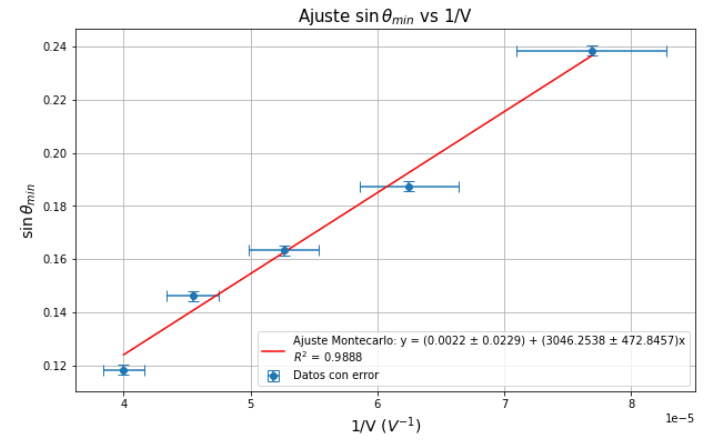
\includegraphics[width=\textwidth]{grafico_2x04_Lif_sin_1_V.png}
  		\caption{\footnotesize Ajuste entre el seno del angulo mínimo al que empieza a emitirse la radiación de frenado, y el inverso del voltaje correspondiente en LiF}
  		\label{fig:Lif_sin_1_V}
  	\end{minipage}
\end{figure}                                                                                                           



\subsection{Estructura cristalina del (KBr). Difractograma}

La segunda muestra analizada es el bromuro de potasio, el cual tiene la misma estructura FCC que  el fluoruro de litio. El difractograma creado a partir de los datos experimentales tomados \ref{fig:difractogramaa_KBr} muestra dos picos de primer orden y también, de forma, clara un pico de $K_{\alpha}$ de orden 2 de difracción. 


\begin{figure}[H]
	\centering
	\begin{minipage}{0.7\textwidth} 
		\includegraphics[width=\textwidth]{grafico_2x03_difractograma_KBr.png}
		\caption{\footnotesize Difractograma de una muestra de bromuro de potasio (BrF) a V=25 kV}
		\label{fig:difractogramaa_KBr}
	\end{minipage}
\end{figure}


De acuerdo a \cite{KBr_quim}, el valor de referencia para la masa molecular del KBr es   $M=119.0$ g$\cdot$ mol$^{-1}$ y el de la densidad $\rho=2.74\text{ g}\cdot\text{cm}^{-3}$. Como en el caso del LiF, aplicando \ref{eq:param_red} obtenemos el parámetro de red, que arroja un valor teórico $a_t=6.607$. El valor encontrado en la bibliografía \cite{KBr_str} para el parametro de red  es $a_b=6.585\pm 0.002$ \AA.

\vspace{\baselineskip}

El valor experimental de la distancia $d$ entre planos atómicos lo calculamos con el promedio de las distancias obtenidas para las tres transiciones principales, con el mismo procedimiento que para el LiF, aunque en esta caso los picos están los suficientemente separados y se usan las energías de transición del cobre \ref{fig:culevels} correspondiente a cada uno de ellos. En la tabla \ref{tab:d_kbr} se muestran los resultados obtenidos.

\vspace{\baselineskip}

\begin{table}[H]
	\centering
	$\Delta \theta = \pm0.1^\circ$ = \pm 0.002 rad; V = 25 Kv\\
	\begin{tabular}{ccccc}
		\toprule
		\toprule
		Transición & Energía (eV) & $\lambda$ (\AA)  &$\theta$ $^\circ$) & $d$ (\AA) \\
		\hline 
		$K_{\alpha_1}$ & 8047.78 & 1.54 &13.2 & 3.373$\pm$0.029 \\
		$K_{\alpha_2}$ & 8027.83 & 3.09 &27.6 & 3.334$\pm$0.013 \\
		$K_{\beta_1}$  & 8905.29 & 1.39 &11.9 & 3.376$\pm$0.032 \\

		\hline
		\hline 
		& & & & \textbf{3.361$\pm$0.025} \\
	\end{tabular}
	\caption{\footnotesize Determinación de la distancia entre planos atómicos en el bromuro de potasio.}
	\label{tab:d_kbr}
\end{table}

\vspace{\baselineskip}

Para el caso del KBr tenemos entonces que $a_t/d = 6.607/3.361 = 1.97 \approx 2 $. De acuerdo a \cite{Cullity2014}, para estructuras FCC com los índices de Miller compatibles son \{200\}. Conocido el plano de difracción es posible hacer una nueva estimación del parámetro de red: $ a_d = 2d = 6.722\pm0.050$ \AA, lo que supone una desviación por exceso entre el 1.3\% y el 2.5\% respecto del valor recogido en la bibliografía.


\section{Discusión}


La comparación de los parámetros de red y distancias interplanares obtenidos experimentalmente para el fluoruro de litio (LiF) y el bromuro de potasio (KBr) con los valores teóricos mostró un buen acuerdo, aunque con ligeras discrepancias. Estas diferencias podrían atribuirse a limitaciones en la resolución del equipo de difracción utilizado o a variaciones en la pureza y preparación de las muestras. Específicamente, el LiF mostró una desviación por exceso de hasta el 1.7\% respecto al valor teórico, mientras que para el KBr, la desviación máxima observada fue del 2.5\%. Estas variaciones están dentro de lo esperable dada la precisión del equipo experimental disponible. Los patrones de difracción observados en este estudio confirmaron las estructuras cristalinas cúbicas centradas en las caras (FCC) para el fluoruro de litio (LiF) y el bromuro de potasio (KBr). Los picos detectados en los difractogramas permitieron calcular las distancias interplanares y los parámetros de la red cristalina aplicando la Ley de Bragg. 

\vspace{\baselineskip}

En cuanto a la estimación de la constante de Planck a partir de los datos de difracción, el valor obtenido estuvo dentro de un margen del 16\% del valor de referencia. Esta variación puede ser significativa, pero es instructiva, indicando la utilidad del método experimental para proporcionar estimaciones razonables en contextos educativos o preliminares, aunque con limitaciones en precisión para aplicaciones más críticas. Las principales fuentes de error parecen derivarse de la precisión en la medición de ángulos y la limitada cantidad de datos disponibles para el ajuste de regresión.



\section{Conclusiones}


En este trabajo  se ha demostrado la capacidad de la difracción de rayos X que, combinada con la Ley de Bragg, ha permitido hacer una estimación de las estructuras cristalinas de compuestos como el fluoruro de litio (LiF) y el bromuro de potasio (KBr). Las estructuras de ambos compuestos se confirmaron como cúbicas centradas en las caras (FCC), y los parámetros de la red calculados desde los datos experimentales coincidieron satisfactoriamente con los valores literarios, validando así las técnicas utilizadas y los modelos teóricos aplicados. La estimación experimental de la constante de Planck, aunque acompañada de una incertidumbre significativa, ilustra la utilidad de la difracción de rayos X como una aproximación válida.


\begin{thebibliography}{99}

\bibitem{LiF_quim}

National Center for Biotechnology Information. (n.d.). PubChem Compound Summary for CID 224478, Lithium fluoride. Retrieved August 19, 2024, from \url{https://pubchem.ncbi.nlm.nih.gov/compound/224478#section=Chemical-and-Physical-Properties}


\bibitem{LiF_str}
Crystallography Open Database. (n.d.). Entry 1010990: Lithium Fluoride (LiF). Retrieved August 19, 2024, from \url{https://www.crystallography.net/cod/1010990.html} 


\bibitem{strlif}
PhysicsOpenLab. Lithium Fluoride (LiF) Crystal. PhysicsOpenLab, 23 January 2018, \url{https://physicsopenlab.org/2018/01/23/lithium-fluoride-lif-crystal/}.

\bibitem{Wahab2021}
Wahab, M. A. Numerical Problems in Crystallography. Springer, 2021

\bibitem{Bearden1967}
Bearden, J. (1967), X-ray wavelengths and x-ray atomic energy levels:, , National Institute of Standards and Technology, Gaithersburg, MD, [online], https://doi.org/10.6028/NBS.NSRDS.14

\bibitem{Haynes2016}
Haynes, W. M. (Ed.). (2016). CRC Handbook of Chemistry and Physics (97th ed.). CRC Press


\bibitem{Cullity2014}
Cullity, B. D., Stock, S. R. (2014). Elements of X-Ray Diffraction. Pearson Education Limited.

\bibitem{KBr_quim}
National Center for Biotechnology Information. PubChem Compound Summary for CID 253877, Potassium Bromide. PubChem, https://pubchem.ncbi.nlm.nih.gov/compound/253877. Accessed 24 Aug. 2024.

\bibitem{KBr_str}
Crystallography Open Database. (n.d.). Entry 1010046: Potassium bromide. Retrieved August 24, 2024, from \url{https://www.crystallography.net/cod/1010046.html}

\end{thebibliography}	


\clearpage


% Tercer artículo
\titleformat{\chapter}[display]
{\normalfont\bfseries}{}{0pt}{\LARGE}
\chapter{Transición de fase en un sistema bidimensional de partículas con potenciales de Lennard-Jones.}
\begin{abstract}
	En este trabajo se ha analiza, mediante diversas simulaciones, el comportamiento de un sistema bidimensional de partículas Argón que interactúan a través del potencial de Lennard-Jones. Estas simulaciones se han realizado con  el programa de simulación Random Phase, para  diversas concentraciones y temperaturas de un sistema de partículas.
\end{abstract}






\section{Introducción}
% ***************************************

El potencial de Lennard-Jones fue formulado por el físico británico John Edward Lennard-Jones en 1924 \cite{Jones1924}. Éste surgió en un contexto histórico en el que la comprensión de las interacciones intermoleculares estaba en sus primeras etapas de desarrollo. Antes de su formulación, las teorías de Van der Waals ya habían destacado la importancia de las fuerzas intermoleculares en los gases reales, lo que llevó a una mejor comprensión de cómo las moléculas interactúan entre sí a diferentes distancias. Sin embargo, las descripciones matemáticas de estas interacciones eran demasiado simples e incapaces de capturar adecuadamente tanto las fuerzas atractivas como las repulsivas.

\vspace{\baselineskip}

Con el objetivo de desarrollar un modelo más preciso, Lennard-Jones combinó una fuerza repulsiva, representada matemáticamente por un término de \( r^{-12} \), y una fuerza atractiva, descrita por un término de \( r^{-6} \). Esta combinación permitió describir de manera efectiva el comportamiento de los átomos y moléculas neutras a distintas distancias, proporcionando una descripción más completa y aplicable a una amplia gama de sistemas. 

\vspace{\baselineskip}

Este potencial es ampliamente utilizado en simulaciones de dinámica molecular debido a su capacidad para capturar las interacciones fundamentales entre átomos y moléculas de manera efectiva y con un costo computacional relativamente bajo. Se aplica en el estudio de la estructura y las propiedades de líquidos, gases y sólidos a nivel microscópico, así como en la exploración de procesos como la adsorción en superficies y la formación de fases cristalinas.



\section{Fundamento teórico}
% ***************************************
\subsection{El potencial de Lennard-Jones}

El potencial de Lennard-Jones es una importante herramienta  en la modelización de las interacciones entre átomos y moléculas neutras. Este potencial se basa en dos componentes básicas que describen el comportamiento de las fuerzas intermoleculares en función de la distancia entre las partículas: una fuerza repulsiva que actúa a distancias muy cortas y una fuerza atractiva que predomina a distancias más largas. Matemáticamente, el potencial se expresa \ref{vlennard}

\begin{equation} \label{vlennard}
	V(r) = 4\epsilon \left[ \left(\frac{\sigma}{r}\right)^{12} - \left(\frac{\sigma}{r}\right)^{6} \right]
\end{equation} 

\vspace{\baselineskip}

 
donde \( r \) es la distancia entre las partículas, \( \epsilon \) representa la profundidad del pozo del potencial, y \( \sigma \) es la distancia a la cual el potencial es cero. La parte repulsiva del potencial, representada por el término \(\left(\frac{\sigma}{r}\right)^{12}\), refleja la fuerte repulsión que ocurre cuando las nubes electrónicas de las partículas comienzan a superponerse.  Por otro lado, el término \(-\left(\frac{\sigma}{r}\right)^{6}\) describe la atracción a distancias más largas.

\vspace{\baselineskip}

El parámetro \( \epsilon \) en la ecuación del potencial determina la profundidad de la atracción entre las partículas, es decir, cuán fuerte es la interacción cuando están a la distancia de equilibrio. Un valor mayor de \( \epsilon \) indica una interacción más fuerte, lo que se traduce en una mayor estabilidad del sistema a esa distancia. Por su parte, \( \sigma \) define la distancia a la cual la fuerza neta entre las partículas es nula, es decir, el punto en el que las fuerzas repulsivas y atractivas se equilibran. Este parámetro está relacionado con el tamaño efectivo de las partículas.


\vspace{\baselineskip}

El comportamiento del potencial de Lennard-Jones se puede entender considerando cómo varía la interacción en función de la distancia. A distancias muy cortas, el término repulsivo domina, haciendo que el potencial se vuelva extremadamente positivo, lo que refleja la repulsión intensa que impide que las partículas se acerquen demasiado. A medida que la distancia aumenta, la atracción empieza a superar la repulsión, alcanzando un mínimo en \( \sigma \), donde las partículas se encuentran en una configuración estable. A distancias aún mayores, el potencial tiende a cero, indicando que la interacción entre las partículas se vuelve insignificante.



\subsection{Algoritmo de Metropolis-Hasting}

Los algoritmos Monte Carlo son una clase de métodos estocásticos que permiten generar secuencias de números aleatorios \(\{X_{i}\}\) siguiendo una distribución de probabilidad específica \(f(X)\). El desarrollo de los métodos de Monte Carlo comineza en la década de 1940 por Stanislaw Ulam y John von Neumann, como una técnica para resolver problemas matemáticos mediante simulaciones aleatorias. 

\vspace{\baselineskip}

Posteriormente, en 1953, Nicholas Metropolis y colaboradores introdujeron el algoritmo de Metropolis \cite{metropolis1953}, un método Monte Carlo específico basado en cadenas de Markov, diseñado para muestrear configuraciones de sistemas físicos. Una cadena de Markov es un proceso estocástico en el cual la probabilidad
de que ocurra un suceso depende sólo y exclusivamente del suceso anterior.

\vspace{\baselineskip}

En 1970, W. K. Hastings generalizó este enfoque con el algoritmo de Metropolis-Hastings \cite{Hastings1970}, ampliando su aplicación a una mayor variedad de distribuciones de probabilidad, lo que lo hizo fundamental en diversos campos científicos

\vspace{\baselineskip}

El algoritmo de Metropolis-Hastings genera un nuevo elemento \(X_{n}\) de la secuencia mediante el siguiente  procedimiento:

\begin{enumerate}
	


\item  Se selecciona un punto de prueba \(X_{p}\) cercano al punto anterior \(X_{n-1}\) y se calcula la razón \ref{eq:razon}

\begin{equation} \label{eq:razon}
	r = \frac{f(X_{p})}{f(X_{n-1})}.
\end{equation} 



\item Si $r > 1$, se acepta el punto de prueba y se asigna $X_{n} = X_{p}$.

\item Si $r < 1$, se acepta el punto con una probabilidad igual a $r$:

	\begin{enumerate}

		\item Se genera un número aleatorio \(\xi\) distribuido uniformemente entre 0 y 1.
		
		\item Si \(\xi < r\), se acepta el punto de prueba y se asigna \(X_{n} = X_{p}\).
		
		\item Si \(\xi > r\), se rechaza el punto de prueba y se mantiene el valor anterior, es decir, \(X_{n} = X_{n-1}\).

	\end{enumerate}
\end{enumerate}

En las simulaciones que emplean el potencial de Lennard-Jones, el algoritmo de Metropolis-Hastings es frecuentemente utilizado para muestrear configuraciones moleculares, donde la probabilidad de aceptar una nueva configuración está dada por un factor proporcional al factor de Boltzmann \ref{eq:fboltzman}

\begin{equation} \label{eq:fboltzman}
	P(E) \propto e^{-\frac{E}{k_{B}T}}
\end{equation}

Este enfoque permite explorar eficientemente el espacio de configuraciones, favoreciendo aquellas con energías más bajas, y es fundamental en simulaciones de dinámica molecular y estudios de propiedades termodinámicas de sistemas basados en el potencial de Lennard-Jones.


\subsection{Parámetro orientacional de una partícula}

El parámetro orientacional  es un parámetro que se empela para describir cómo las partículas se orientan en relación con sus vecinas más cercanas. Este parámetro permite identificar transiciones de fase, como la transición de un líquido a un sólido, donde se espera que las partículas en la fase sólida muestren un mayor grado de alineación o simetría en sus orientaciones. En general, se basa en la comparación de ángulos entre las posiciones relativas de las partículas vecinas.

\vspace{\baselineskip}

Matemáticamente,el parámetro orientacional de la partícula \( m \) se define por \ref{eq:parpos}.

\begin{equation} \label{eq:parpos}
	\vec{\Psi}_{m} = \sum_{j=1}^{n_{m}} e^{6i\theta_{mj}}
\end{equation}

donde \( n_{m} \) es el número de vecinos más próximos a la partícula \( m \) y \( \theta_{mj} \) es el ángulo que forma el vector que conecta las partículas \( m \) y \( j \) con respecto al eje \( X \). El módulo de este vector, \( |\vec{\Psi}_{m}| \), proporciona una medida del grado de orden en la distribución de los vecinos más cercanos, permitiendo caracterizar la estructura local de la red de partículas. Específicamente:

\begin{itemize}

	\item \( |\vec{\Psi}_{m}| = 1 \) indica que los vecinos más próximos están organizados en una red triangular, lo cual es característico de una fase sólida con simetría hexagonal.
	\item \( 0 < |\vec{\Psi}_{m}| < 1 \) sugiere una distribución irregular de los vecinos, lo que indica un cierto grado de desorden en la estructura local.
	\item \( |\vec{\Psi}_{m}| = 0 \) implica que los vecinos siguen un patrón distinto al de una red triangular, como en el caso de una fase líquida o una estructura amorfa.

\end{itemize}

Este parámetro es fundamental en el análisis de transiciones de fase y en la caracterización del orden local en sistemas simulados con potenciales como el de Lennard-Jones.

\section{Generación de simulaciones}

Para llevar cabo las simulaciones se ha utilizado el software Random Phase \cite{rf2022}. Estas simulaciones se llevarán a cabo para 1000 partículas con diferentes casuísticas de concentración de partículas y temperatura. 


\subsection{Simulación 1: $\rho = 0.001$ \AA$^{-2}$, T = 1 K}

En esta simulación, la distribución espacial de las partículas (Figura \ref{fig:d001t1}), muestra un sistema altamente diluido con partículas dispersas en todo el espacio de simulación. La mayoría de las partículas se encuentran aisladas, pero se observan algunos pares y pequeños grupos, indicativos de la formación de dímeros y clusters transitorios. El parámetro orientacional, representado por el color de los puntos, muestra que algunas partículas forman estructuras locales ordenadas (puntos azules), mientras que la mayoría no presenta una orientación preferente (puntos grises), característico de un estado gaseoso.

\vspace{\baselineskip}

La función de distribución radial $g(r)$, presentada en la figura \ref{fig:rdf001t1}, muestra tres picos característicos:	

\begin{enumerate}
	
\item El primer pico, muy pronunciado, aparece a aproximadamente 3.8 Å. Este pico corresponde a la distancia de equilibrio del potencial de Lennard-Jones y está directamente relacionado con el parámetro $\sigma$ del potencial. La explicación de este máximo se deriva de la forma del potencial de Lennard-Jones. Con $\sigma=3.4$ Å, el potencial muestra un mínimo alrededor de $r \approx 3.8$ Å, como se demuestra en \ref{eq:maxjones}.
	
\begin{equation} \label{eq:maxjones}
		x = \left(\frac{\sigma}{r}\right)^{6} \rightarrow V(x) = \epsilon\cdot(x^2-x); \quad V'(x) = 0 \rightarrow x=\frac{1}{2} \rightarrow r_0=2^{1/6}\sigma \approx 3.8 \text{ Å}  
\end{equation}
	
Las partículas más próximas tienden a agruparse en el fondo del pozo de potencial, acercándose a esta distancia específica y formando agrupaciones en forma de triángulo equilátero de lado $r_0$. Debido a la baja temperatura, las partículas carecen de la energía necesaria para moverse lejos de esta posición.
	
\item Un segundo pico, más débil, aparece alrededor de 6.6 Å. Esta distancia es aproximadamente $\sqrt{3}$ veces la distancia del primer pico, lo que sugiere la formación de configuraciones similares a rombos o triángulos equiláteros. Eventualmente, alguna otra partícula podría caer en las inmediaciones de una agrupación triangular y formar un rombo de lado $r_0$, cuya diagonal mayor vendría dada por $r_1=\sqrt{3}r_0\approx 6.6$ Å.
	
\item Un tercer pico, aún más débil, se observa a 7.6 Å $\approx 2r_0$. Este pico no encaja a priori con agregaciones basadas en triángulos equiláteros, siendo esta distancia compatible con interacciones entre agrupaciones fuera de la vecindad inmediata o con clústeres lineales.
	
\end{enumerate}

\begin{figure}[H]
	\centering
	% Imagen (a) con factor de escala del 80%
	\begin{minipage}[b]{0.45\textwidth}
		\centering
		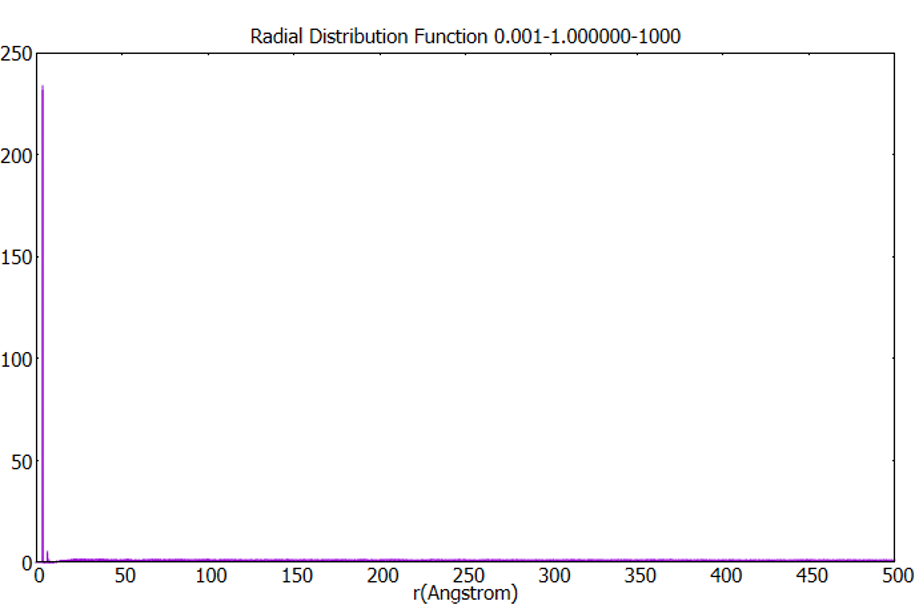
\includegraphics[width=0.95\textwidth]{grafico_3x01_0.001-1.png} % Ajusta 0.8 al factor deseado
		\textbf{(a)}
		\vspace{0.75cm}
	\end{minipage}%
	\hfill
	% Imagen (b) con factor de escala del 100%
	\begin{minipage}[b]{0.45\textwidth}
		\centering
		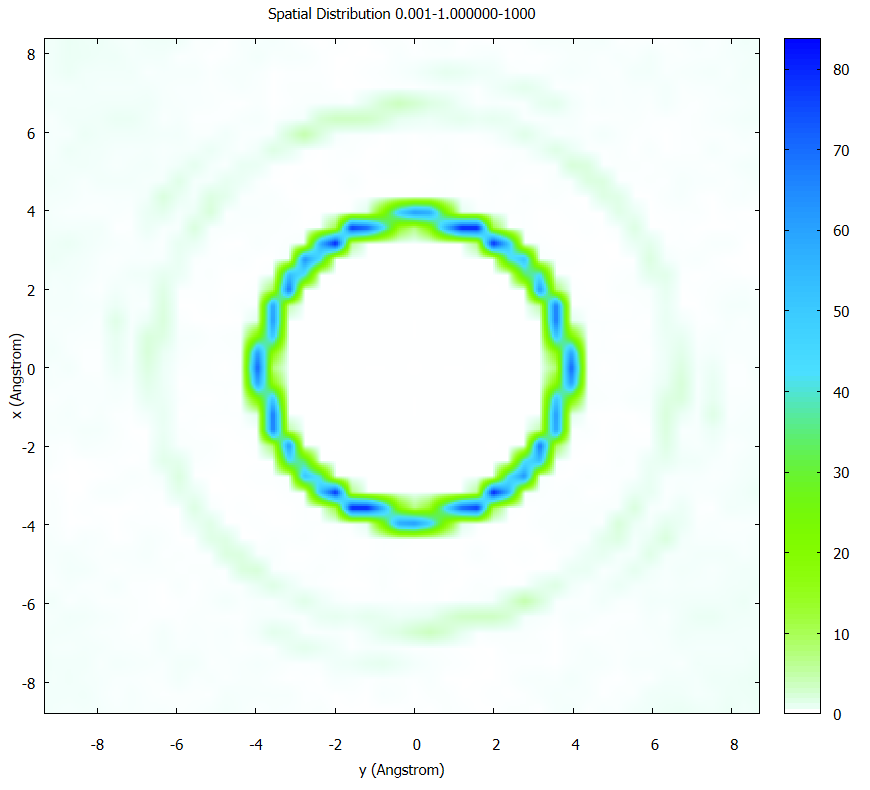
\includegraphics[width=0.95\textwidth]{grafico_3x05_0.001-1_distribucion.png} % Ajusta 1.0 al factor deseado
		\textbf{(b)}
	\end{minipage}
	
	
	% Imagen (c) con factor de escala del 90%
	\begin{minipage}[b]{0.45\textwidth}
		\centering
		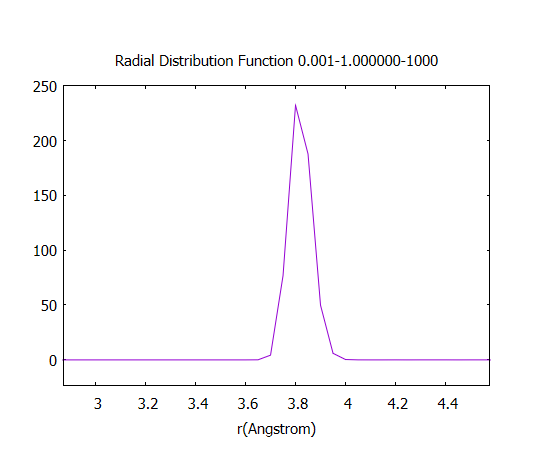
\includegraphics[width=\textwidth]{grafico_3x02_0.001-1_zoom.png} % Ajusta 0.9 al factor deseado
		\textbf{(c)}
	\end{minipage}%
	\hfill
	% Imagen (d) con factor de escala del 70%
	\begin{minipage}[b]{0.45\textwidth}
		\centering
		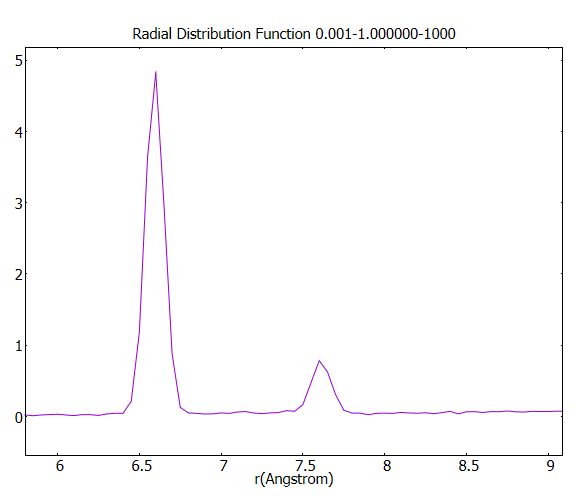
\includegraphics[width=0.95\textwidth]{grafico_3x03-0.001_1_minipico.png} % Ajusta 0.7 al factor deseado
		\textbf{(d)}
	\end{minipage}
	\caption{\footnotesize Simulación $\rho=$ 0,001 partículas $\cdot$ \AA$^{-2}$ y  T=1 K. a) Gráfica general de distribución radial (RDF). b) Distribución  radial. c)  y d) Detalles de la distribución radial donde se observan dos máximos locales en 3.8 \AA {} y de 6.6 \AA {} y 7.6 \AA {} respectivamente.}
	\label{fig:rdf001t1}
\end{figure}
	
\vspace{\baselineskip}
	
La rápida caída de $g(r)$ después del primer pico y su aproximación a 1 para distancias mayores indica la ausencia de estructura de largo alcance, confirmando el estado gaseoso del sistema. Sin embargo, la presencia de los picos secundarios sugiere que ocasionalmente se forman agrupaciones un poco más grandes, probablemente de 3 o 4 partículas, aunque estas son muy transitorias debido a la baja densidad. Esto se muestra claramente en la figura \ref{fig:d001t1}
	
\vspace{\baselineskip}
	
La distribución espacial promedio exhibe una simetría radial, lo que confirma la naturaleza isotrópica del sistema, típica de un gas. Esta simetría indica que no hay direcciones preferentes para la formación de agrupaciones, y las partículas se mueven libremente en todas las direcciones.
	
\vspace{\baselineskip}
	
En conjunto, estos resultados son consistentes con un sistema en estado gaseoso muy diluido a baja temperatura. Las interacciones de Lennard-Jones son evidentes a cortas distancias, permitiendo la formación de dímeros y pequeños clusters transitorios, pero el sistema mantiene en general las características de un gas. 
	

\begin{figure}[H]
	\centering
	\begin{minipage}[b]{0.42\textwidth}
		\centering
		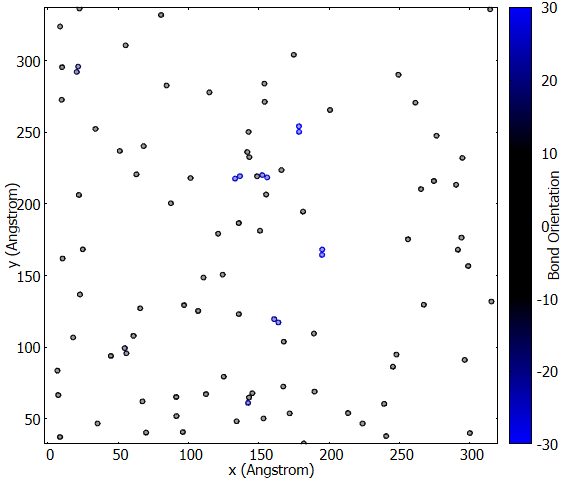
\includegraphics[width=1\textwidth]{grafico_3x04_0.001-1_dinamica.png}
		\textbf{(a)}
	\end{minipage}%
	\hfill
	\begin{minipage}[b]{0.45\textwidth}
		\centering
		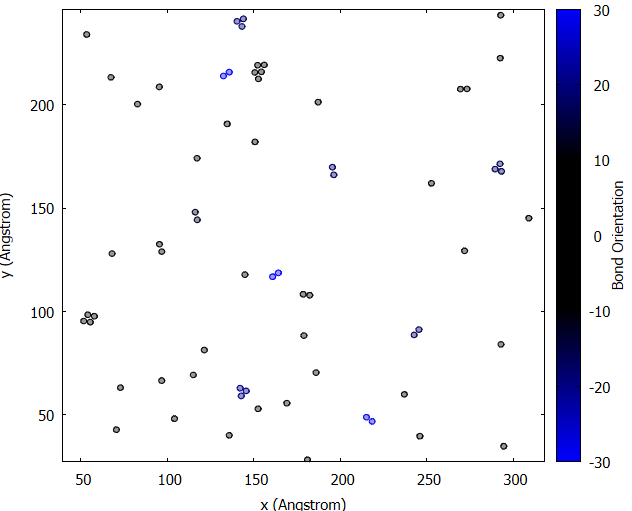
\includegraphics[width=1\textwidth]{grafico_3x06_0.001-1_dinamica_zoom.png}
		\textbf{(b)}
	\end{minipage}
	
	\caption{\footnotesize Simulación  $\rho=$ 0,001 \AA$^{-2}$ y  T=100 K. a) Disposición espacial de las partículas obtenida al final de la simulación y detalle del mismo b).}
	\label{fig:d001t1}
\end{figure}

\subsection{Simulación 2: $\rho = 0.001$ \AA$^{-2}$, T = 100 K}

En esta caso aparece, en la RDF, figura \ref{fig:d001t100}a, aparece un único pico para una distancia de alrededor de 3.8 \AA, correspondiente a la distancia de equilibrio del potencial de Lennard-Jones. Sin embargo, este pico es bajo y muestra un ensanchamiento significativo. Después de este pico principal, $g(r)$ decae rápidamente y se aproxima a 1 para distancias mayores a 6 \AA, sin mostrar picos secundarios claramente definidos.

\vspace{\baselineskip}
	
La distribución espacial de las partículas, mostrada en la Figura \ref{fig:d001t100}b), presenta un sistema altamente diluido con partículas dispersas uniformemente en todo el espacio de simulación. La gran mayoría de las partículas aparecen como puntos grises aislados, indicando la ausencia de una orientación preferente. Se observan muy pocos partículas azules, lo que sugiere que la formación de estructuras locales ordenadas es un fenómeno raro en estas condiciones.

\begin{figure}[H]
	\centering
	\begin{minipage}[b]{0.475\textwidth}
		\centering
		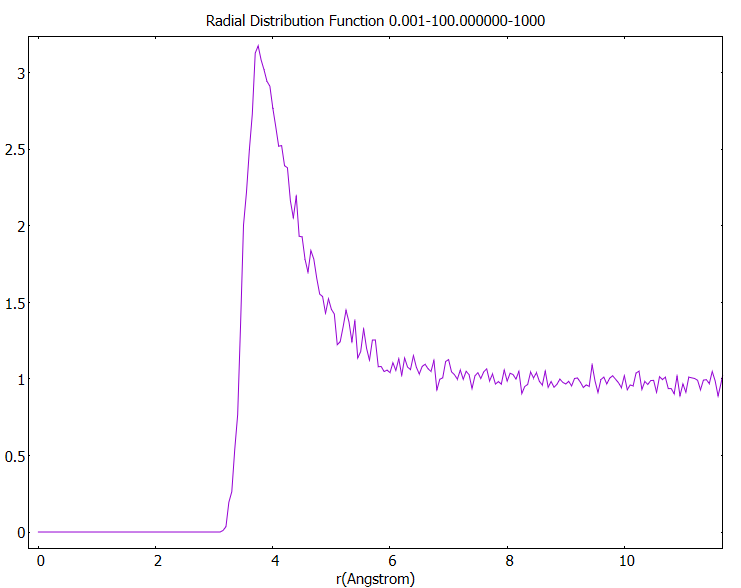
\includegraphics[width=\textwidth]{grafico_3x07_0.001-100_rdf_zoom.png}
		\textbf{(a)}
	\end{minipage}%
	\hfill
	\begin{minipage}[b]{0.45\textwidth}
		\centering
		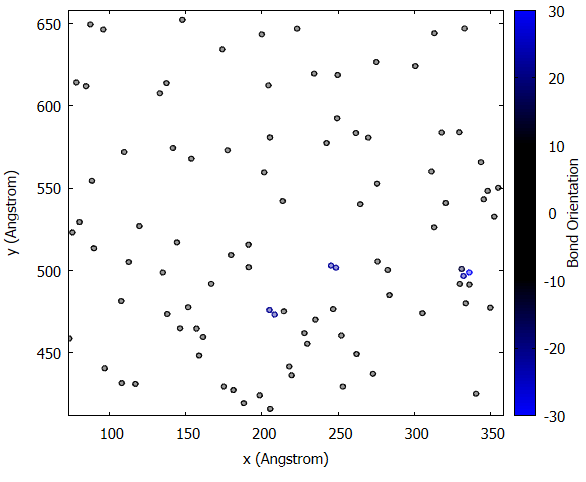
\includegraphics[width=\textwidth]{grafico_3x06_0.001-100_dinamica_zoom.png}
		\textbf{(b)}
	\end{minipage}
	
	\caption{\footnotesize Simulación  $\rho=$ 0.001 \AA$^{-2}$ y  T=100 K. a) Único máximo a 3.8 \AA en la función de distribución radial b) Disposición de las partículas en su vecindad.}
	\label{fig:d001t100}
\end{figure}
	
Estas observaciones apuntan a un sistema que se comporta de manera muy similar a un gas ideal. La baja altura y el ensanchamiento del primer pico en $g(r)$ indican que las interacciones de Lennard-Jones, aunque presentes, tienen un efecto relativamente débil en la estructura del sistema. La rápida convergencia de $g(r)$ a 1 para distancias mayores sugiere que no hay correlaciones de largo alcance entre las partículas.

\vspace{\baselineskip}
	
Comparando con la simulación 1, la alta temperatura proporciona a las partículas una energía cinética significativa, permitiéndoles superar fácilmente las atracciones de corto alcance. Esto resulta en una distribución más uniforme de las partículas y una menor tendencia a formar agrupaciones estables. La formación de dímeros o pequeños clusters es muy poco frecuente debido a la alta energía térmica del sistema.
	
	




\subsection{Simulación 3: $\rho = 0.01$ \AA$^{-2}$, T = 1 K}


En este caso la distribución espacial de las partículas, Figura \ref{fig:0.01t1}a, revela un sistema con una estructura altamente organizada. Se observan numerosas agrupaciones de partículas, predominantemente en forma de triángulos equiláteros y estructuras más complejas derivadas de estos. Los puntos azules y negros indican diferentes orientaciones locales de estas estructuras.

\vspace{\baselineskip}

La función de distribución radial $g(r)$, presentada en la Figura \ref{fig:0.01t1}b, muestra una serie de picos agudos y bien definidos. El primer pico, extremadamente pronunciado, aparece a aproximadamente 3.8 Å, correspondiente a la distancia de equilibrio del potencial de Lennard-Jones. La altura de este pico, cercana a 115, indica una fuerte correlación entre pares de partículas a esta distancia.

\begin{figure}[H]
	\centering
	\begin{minipage}[b]{0.4\textwidth}
		\centering
		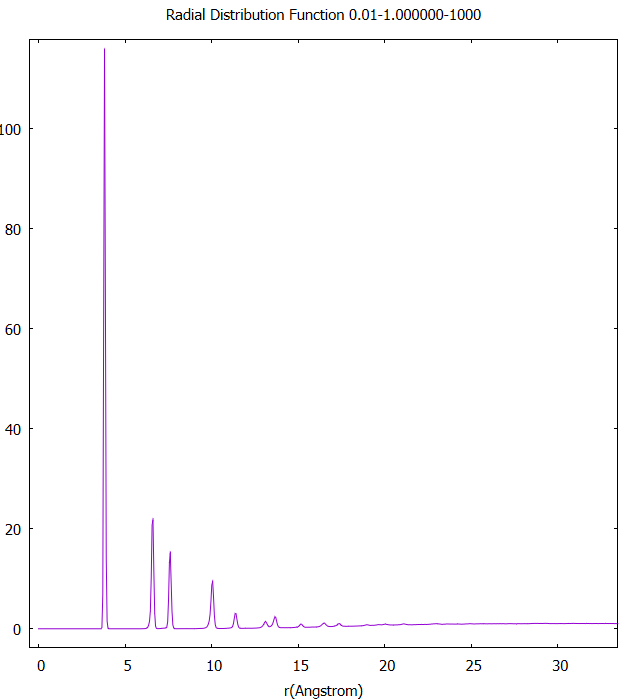
\includegraphics[width=1\textwidth]{grafico_3x08_0.01_1_rdf.png}
		\textbf{(a)}
	\end{minipage}%
	\hfill
	\begin{minipage}[b]{0.5\textwidth}
		\centering
		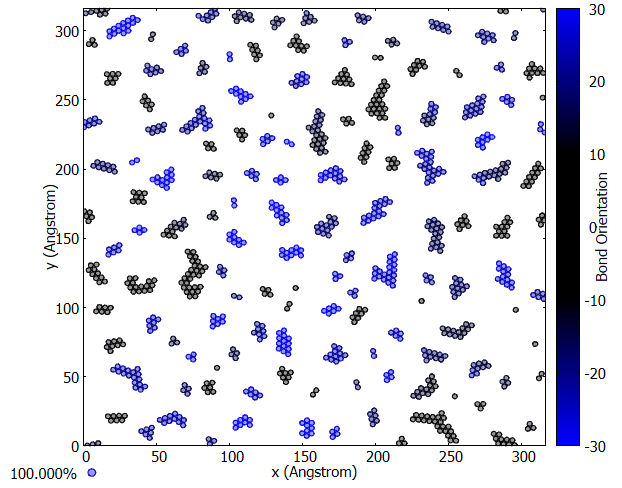
\includegraphics[width=1\textwidth]{grafico_3x09_0.01_1_dinamica.png}
		\textbf{(b)}
	\end{minipage}
	
	\caption{\footnotesize Simulación  $\rho=$ 0.01 \AA$^{-2}$ y  T=1 K. a) Función de distribución radial. Sucesión de máximos para diferentes distancias. b) Agregados de  partículas  obtenidos al final  de la simulación.}
	\label{fig:0.01t1}
\end{figure}

Se observan picos secundarios claros y distintos a distancias mayores, resaltando los situados a 6.6, 7.6 y 10 \AA. Estos picos corresponden a las distancias características en las estructuras triangulares y sus derivados que ya hemos visto previamente, a excepción de la correspondiente a 10 \AA, que surge de las diversas agregaciones de segundo orden entre estructuras romboidales y/o triangulares. La presencia de múltiples picos bien definidos en $g(r)$ hasta distancias relativamente grandes sugiere un alto grado de orden estructural en el sistema. Esto es consistente con la formación de clusters grandes y estables, como se observa en la figura \ref{fig:0.01t1}b.

\vspace{\baselineskip}

El sistema muestra características de una fase intermedia entre líquido y sólido, posiblemente un líquido altamente estructurado o una fase cristalina con defectos. La baja temperatura permite que las interacciones de Lennard-Jones dominen sobre la agitación térmica, resultando en la formación de estructuras ordenadas extensas.






\subsection{Simulación 4: $\rho = 0.01$ \AA$^{-2}$, T = 100 K}

La distribución espacial de las partículas, mostrada en la figura \ref{fig:0.01t100}b, presenta un sistema mucho menos estructurado en comparación con T=1 K, de la simulación 4. Las partículas están distribuidas de manera más uniforme en todo el espacio de simulación, con una disminución notable en la formación de agrupaciones estables. La mayoría de las partículas aparecen como puntos grises aislados, indicando la ausencia de una orientación preferencial.

\vspace{\baselineskip}

La función de distribución radial $g(r)$, figura \ref{fig:0.01t100}a, muestra cambios importantes en comparación con la simulación previa. El primer pico, aunque todavía visible, es mucho menos pronunciado y más ancho, con una altura máxima de aproximadamente 2.9. Este pico aparece alrededor de 3.8 \AA, correspondiente a la distancia de equilibrio del potencial de Lennard-Jones, pero su menor altura y mayor anchura indican interacciones más débiles y transitorias entre pares de partículas.  

\vspace{\baselineskip}

Después del primer pico, $g(r)$ decae rápidamente y se aproxima a 1, con debil 'hombro' próximo a 8 \AA que podría indican la formación ocasional de estructuras más grandes que pueden apreciarse en la figura \ref{fig:0.01t100}b. La ausencia de picos secundarios claros sugiere que no hay estructuras ordenadas de largo alcance en el sistema.  

\vspace{\baselineskip}

Estas observaciones indican que el sistema se comporta de manera muy similar a un gas denso. La temperatura proporciona a las partículas una energía cinética significativa, permitiéndoles superar fácilmente las atracciones de corto alcance del potencial de Lennard-Jones. Esto resulta en una distribución más uniforme de las partículas y una menor tendencia a formar agrupaciones estables.



\begin{figure}[H]
	\centering
	\begin{minipage}[b]{0.47\textwidth}
		\centering
		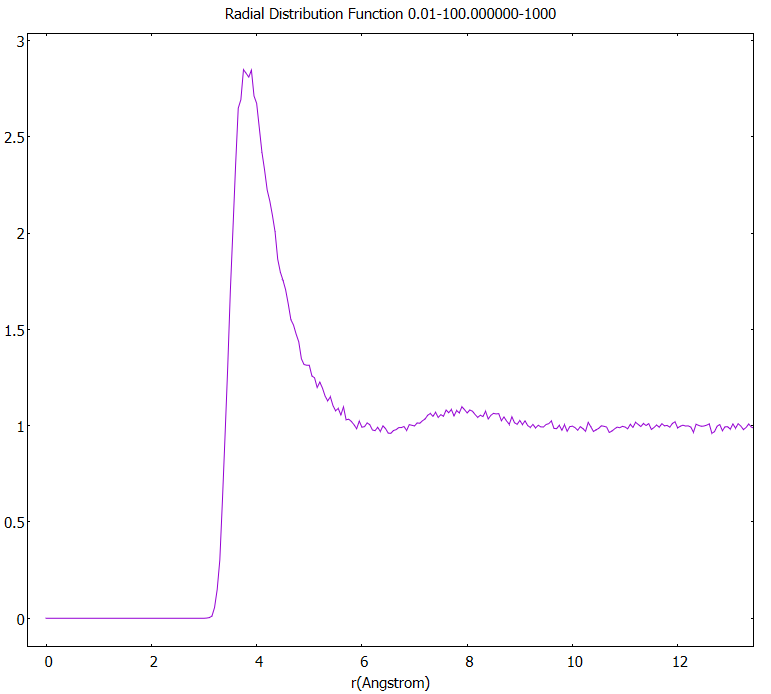
\includegraphics[width=1\textwidth]{grafico_3x11_0.01_100_rdf.png}
		\textbf{(a)}
	\end{minipage}%
	\hfill
	\begin{minipage}[b]{0.5\textwidth}
		\centering
		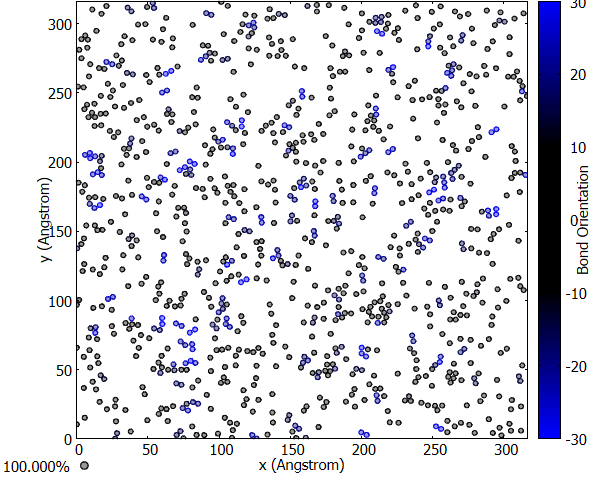
\includegraphics[width=1\textwidth]{grafico_3x10_0.01_100_dinamica.png}
		\textbf{(b)}
	\end{minipage}
	
	\caption{\footnotesize Simulación  $\rho=$ 0.01 \AA$^{-2}$ y  T=100 K. a) Función de distribución radial.  b) Agregados de  partículas  obtenidos al final de la simulación.}
	\label{fig:0.01t100}
\end{figure}


\subsection{Simulación 5: $\rho = 0.05$ \AA$^{-2}$, T = 1 K}


En este caso el sistema exhibe una estructura predominantemente cristalina. La distribución espacial, figura \ref{fig:0.05t1}b, muestra una red consistente con una estructura hexagonal y con grandes regiones con una fuerte orientación local. Esta red se compone de triángulos equiláteros que forman rombos y estructuras más complejas. 

\vspace{\baselineskip}
	
La función g(r) a T=1, figura \ref{fig:0.05t1}a,  confirma esta disposición ordenada. Un pico agudo y prominente cerca de 3.8 \AA, seguido de múltiples picos secundarios bien definidos hasta largas distancias, indica un orden de largo alcance típico de los cristales. En estas condiciones, las interacciones de Lennard-Jones predominan sobre la agitación térmica, generando esta configuración altamente organizada.


\begin{figure}[H]
	\centering
	\begin{minipage}[b]{0.47\textwidth}
		\centering
		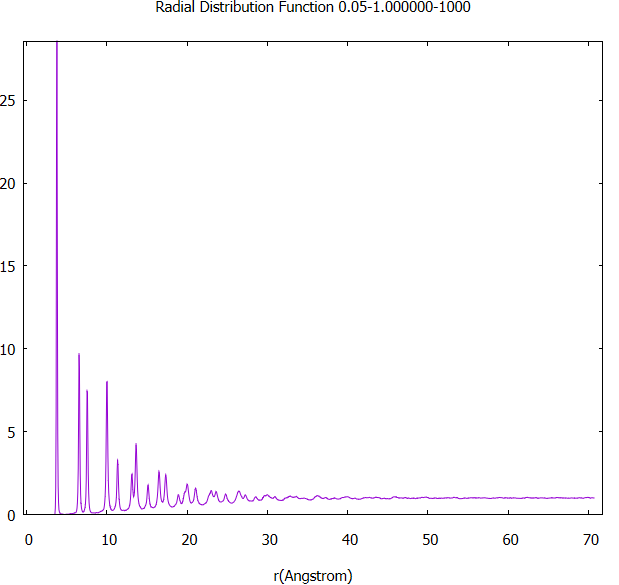
\includegraphics[width=1\textwidth]{grafico_3x12_0.05_1_rdf.png}
		\textbf{(a)}
	\end{minipage}%
	\hfill
	\begin{minipage}[b]{0.5\textwidth}
		\centering
		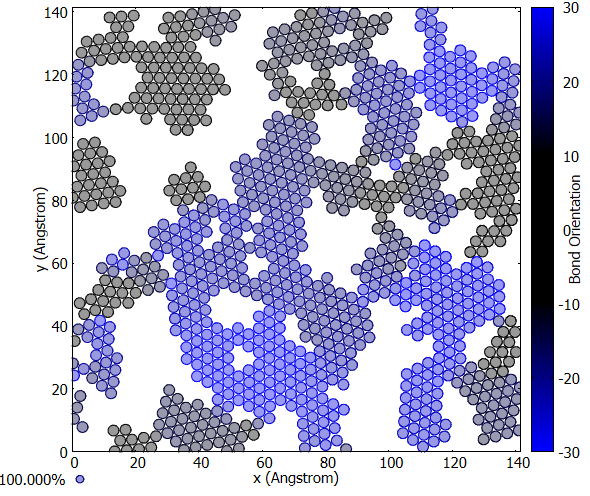
\includegraphics[width=1\textwidth]{grafico_3x13_0.05_1_dinamica.png}
		\textbf{(b)}
	\end{minipage}
	
	\caption{\footnotesize Simulación  $\rho=$ 0.05 \AA$^{-2}$ y  T=1 K. a) Función de distribución radial. Sucesión de máximos para diferentes distancias. b) Agregados de  partículas  obtenidos al final de la simulación. Estructura predominantemente cristalina.}
	\label{fig:0.05t1}
\end{figure}

\subsection{Simulación 6: $\rho = 0.05$ \AA$^{-2}$, T = 100 K}

En este caso la estructura cambia bastante respecto a la simulación 5. La distribución espacial, figura \ref{fig:0.05t100}b ya no muestra una estructura cristalina. En su lugar, se observa una mezcla de partículas con orientaciones variadas. Hay presencia de pequeños grupos y pares de partículas, pero no se ven estructuras ordenadas grandes. La función $g(r)$, figura \ref{fig:0.05t100}a,  presenta un primer pico más bajo y ancho que a T=1 K y varios picos adicionales de menor entidad convergiendo posterior mente a $g(r)=1$ con la distancia. Esto picos tienen sus homólogos a la misma distancia $r$, aunque para T=1, se presentan muchos mas picos adicionales. 


\begin{figure}[H]
	\centering
	\begin{minipage}[b]{0.45\textwidth}
		\centering
		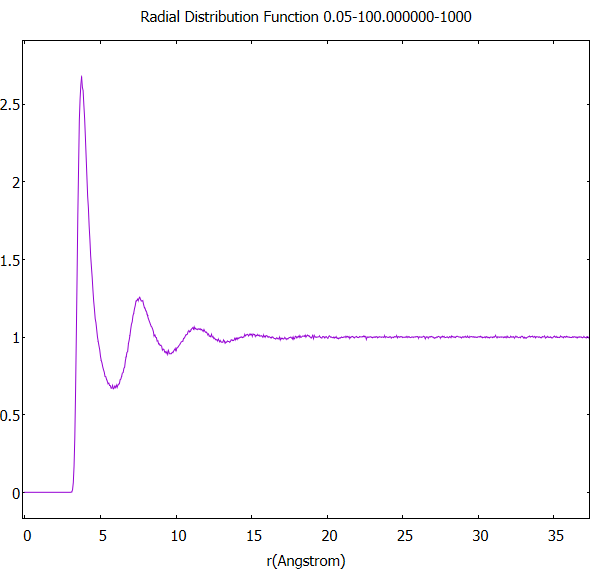
\includegraphics[width=1\textwidth]{grafico_3x14_0.05_100_rdf.png}
		\textbf{(a)}
	\end{minipage}%
	\hfill
	\begin{minipage}[b]{0.5\textwidth}
		\centering
		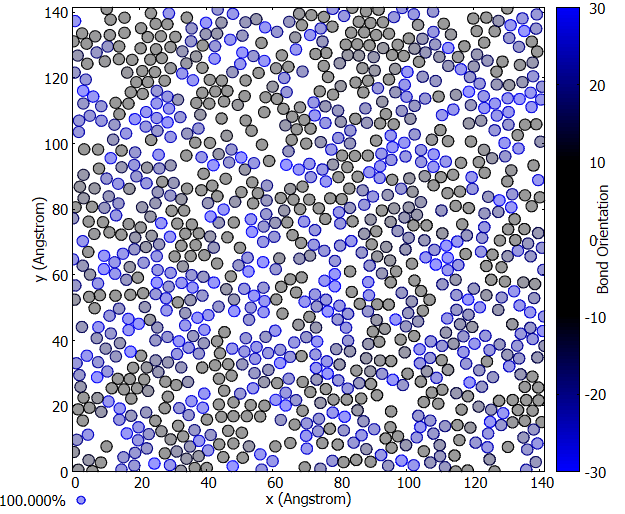
\includegraphics[width=1\textwidth]{grafico_3x15_0.05_100_dinamica.png}
		\textbf{(b)}
	\end{minipage}
	
	\caption{\footnotesize Simulación  $\rho=$ 0.05 \AA$^{-2}$ y  T=100 K. a) Función de distribución radial. Disminución del número de máximos para diferentes distancias la aumentar la temperatura. b) Agregados de  partículas  obtenidos al final al final de la simulación.}
	\label{fig:0.05t100}
\end{figure}

\subsection{Simulaciones 7,8 y 9: $\rho = 0.1$ \AA$^{-2}$, T = 1 K, T =100, T=1000}
En las simulaciones descritas anteriormente,  hemos visto que las partículas interactúan a través del potencial de Lennard-Jones, cuyo mínimo se encuentra a una distancia $r\approx=3.81$ \AA. Este es el punto donde la atracción y la repulsión se equilibran, dando lugar a la menor energía posible entre las partículas. No obstante en la simulaciones a para $\rho=0.1$ \AA$^{-2}$, los picos priméros máximos de g(r) obtenidos no coinciden exactamente con este valor (o múltiplos) Esto se debe a que, además del mínimo del potencial, las interacciones térmicas y el empaquetamiento local afectan la organización de las partículas.

\vspace{\baselineskip}

En un sistema de esferas duras, el empaquetamiento compacto se refiere al máximo de densidad alcanzable cuando las partículas están en contacto directo. En un sistema tridimensional ideal, como en el empaquetamiento cúbico centrado en las caras (FCC), se alcanza una densidad de aproximadamente 74\%. En contraste, en un sistema bidimensional, un empaquetamiento hexagonal ideal logra una densidad cercana al 90.69\%

\begin{figure}[H]
	\centering
	\begin{minipage}[b]{0.38\textwidth}
		\centering
		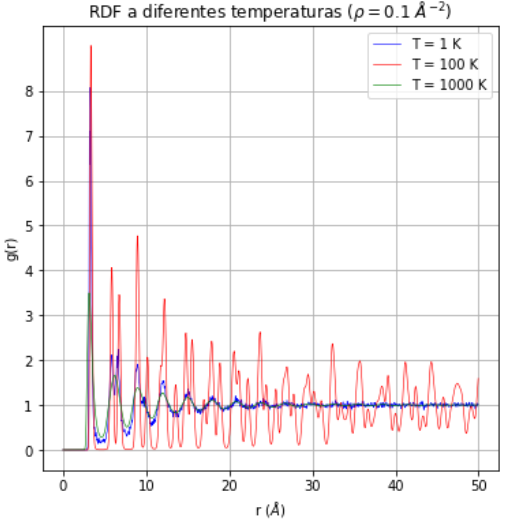
\includegraphics[width=1\textwidth]{grafico_3x17_0.1_rdf.png}
		\textbf{(a)}
	\end{minipage}%
	\begin{minipage}[b]{0.62\textwidth}
		\centering
		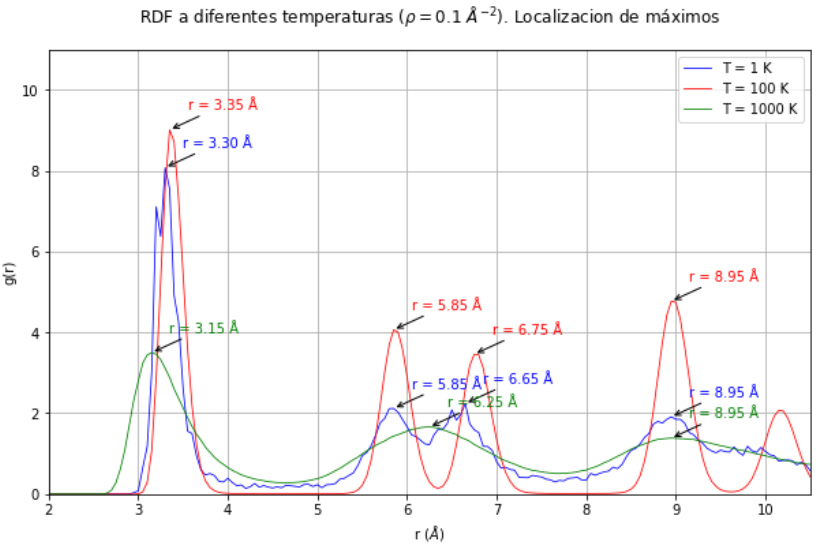
\includegraphics[width=1\textwidth]{grafico_3x16_0.1_rdf_detalle.png}
		\textbf{(b)}
	\end{minipage}
	\caption{\footnotesize Simulación  $\rho=$ 0.1 \AA$^{-2}$. a) Funciones de distribución radial para T=1, 100 y 1000 K. b) Detalle de RDF con las distancias donde se producen los picos de g(r).}
	\label{fig:rdf_0.1}
\end{figure}

\vspace{\baselineskip}

Los mínimos observados en la RDF \ref{fig:rdf_0.1} a distancias menores que 3.81 \AA{} son compatible con el hecho de que una densidad alta de partículas ,incluso a bajas temperaturas, pueden dar lugar a configuraciones de energía, figura \ref{fig:energiasxx} estables a distancias inferiores al mínimo del potencial de Lennard-Jones. A medida que la temperatura aumenta, el sistema se vuelve más desordenado y la distancia de los mínimos en la RDF se aleja del valor de 3.81 \AA, ya que la energía térmica adicional permite mayores fluctuaciones en las energías y posiciones que originan nuevas configuraciones estables, si bien menos probables si nos atenemos a la evolución de los picos en g(r).


\begin{figure}[H]
	\centering
	\begin{minipage}[b]{0.60\textwidth}
		\centering
		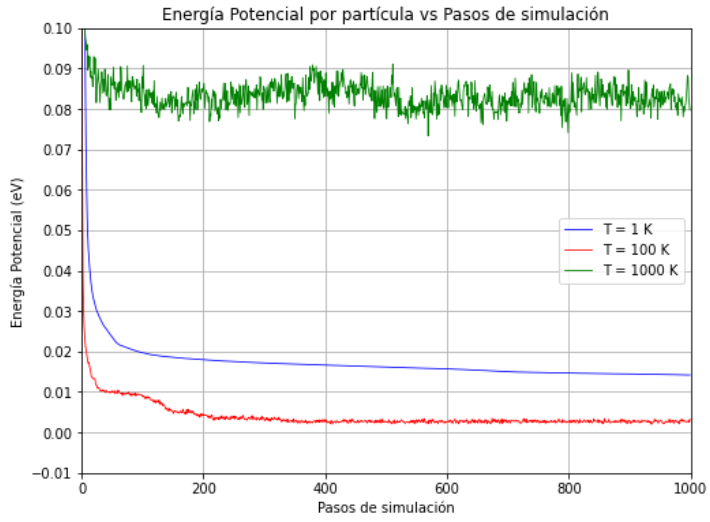
\includegraphics[width=1\textwidth]{grafico_3x18_0.1_energias_detalle.png}
		\caption{\footnotesize Simulación  $\rho=$ 0.1 \AA$^{-2}$.Evolución de la energía potencial al avanzar la simulación para las temperaturas: T=1, 100 y 1000 K.}
		\label{fig:energiasxx}
	\end{minipage}%
\end{figure}


Los diagramas de Voronoi, figura \ref{fig:voronoi},  permiten visualizar la estructura local del sistema y cómo esta cambia con la temperatura. 

\vspace{\baselineskip}

A T= 1 K, el sistema muestra una estructura cristalina casi perfecta, con muy pocos defectos. Esto se alinea con la función g(r) que mostraba picos agudos y bien definidos, y con la baja energía potencial observada. La uniformidad en la orientación de los enlaces y el alto módulo de orientación confirman el alto grado de orden estructural.

\begin{figure}[H]
	\centering
	\begin{minipage}[b]{0.9\textwidth} % Ajusta la anchura según necesites
		\centering
		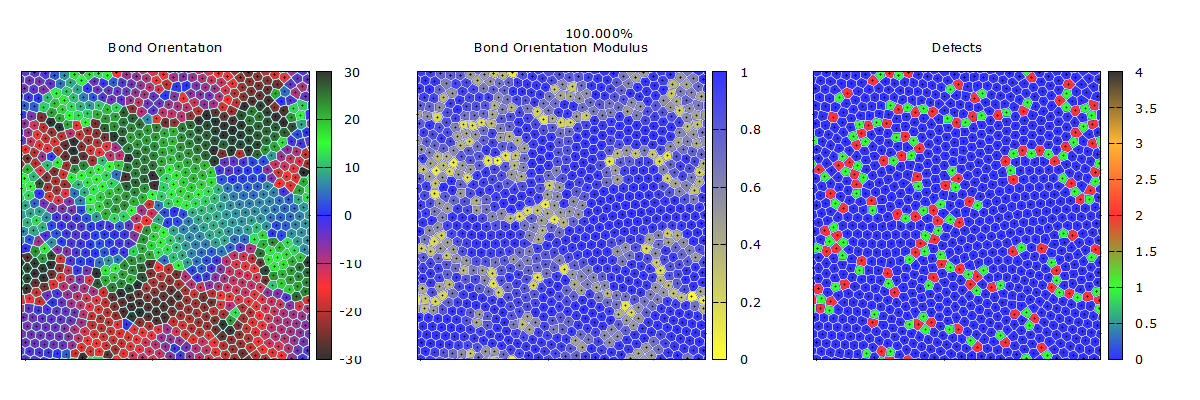
\includegraphics[width=1\textwidth]{grafico_3x19_voronoi_T1.png}
		\textbf{(a)}
	\end{minipage}
	
	\begin{minipage}[b]{0.9\textwidth} % Ajusta la anchura según necesites
		\centering
		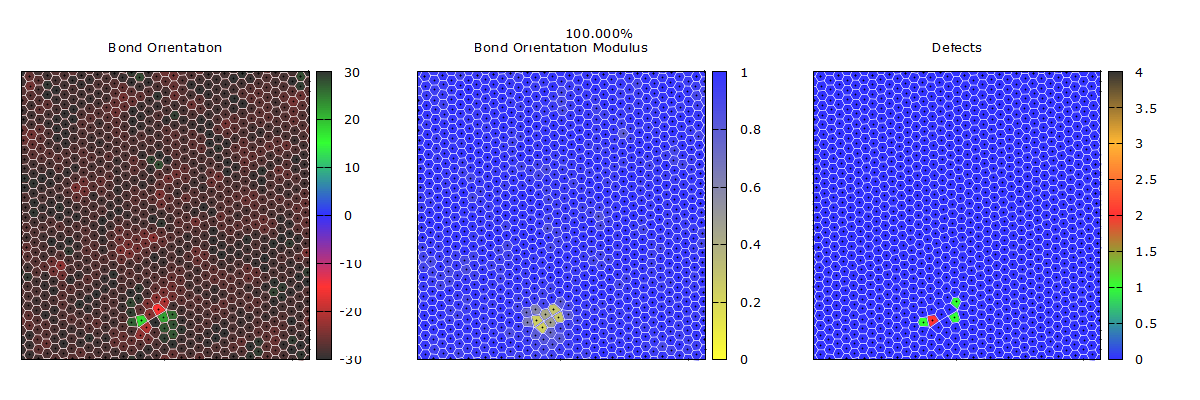
\includegraphics[width=1\textwidth]{grafico_3x20_voronoi_T100.png}
		\textbf{(b)}
	\end{minipage}
	
	\begin{minipage}[b]{0.9\textwidth} % Ajusta la anchura según necesites
		\centering
		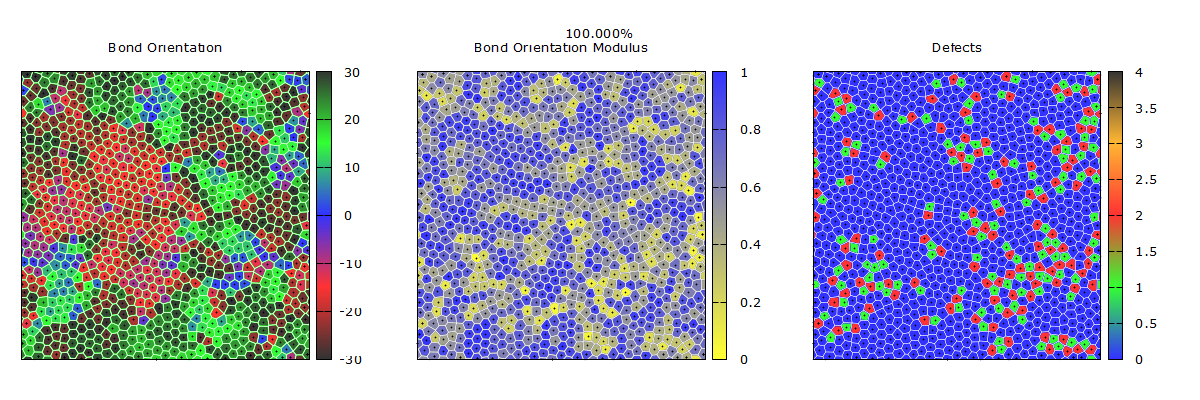
\includegraphics[width=1\textwidth]{grafico_3x21_voronoi_T1000.png}
		\textbf{(b)}
	\end{minipage}
	
	\caption{\footnotesize a) Diagramas de Voronoi al final de la simulación para T=1, 100 y 1000 K}
	\label{fig:voronoi}
\end{figure}



Para T=100 K se observa que hay regiones con orden local significativo, pero también algunas áreas más desordenadas. Esto podría explicar la observación de una energía potencial más baja que a T = 1K. El sistema ha ganado suficiente energía térmica para superar barreras locales y explorar configuraciones que, en promedio, resultan en una energía más baja. Los defectos, aunque presentes, están más organizados,  y posiblemente contribuyendo a esta optimización energética. Esto es sugiere la existencia de un estado intermedio complejo a T = 100K, donde el sistema parece encontrar un equilibrio óptimo entre orden estructural y minimizar la energía.


\vspace{\baselineskip}


A T=100 K el sistema muestra un alto grado de desorden, consistente con un estado líquido o gas denso. Sin embargo, la presencia de algunas regiones con orden local (vistas en el módulo de orientación de enlaces) explica la persistencia de picos en g(r) a esta alta temperatura. Los numerosos defectos dispersos confirman la alta energía potencial y las fluctuaciones observadas.


\subsection{Análisis del proceso de termalización}

Realizadas todas la simulaciones una de las cuestiones a determinar es si el proceso de termalización ha sido lo bastante largo como para llegar al equilibrio. En la gráfica \ref{fig:termal} se muestra la  evolución de la energía potencial por partícula para densidades de partículas a T=1 K empleadas en las simulaciones. De su análisis  se extrae  que el proceso de termalización ha sido suficientemente extenso para alcanzar el equilibrio en todos los casos estudiados. De un lado se observa una rápida caída inicial de la energía en los primeros pasos, seguida de una estabilización significativa después de 200-300 pasos.Además la última mitad de la simulación muestra curvas prácticamente planas con fluctuaciones mínimas, indicando que se ha alcanzado un estado de equilibrio estable.

\vspace{\baselineskip}

Aunque las densidades más altas parecen requerir un tiempo de equilibrio ligeramente mayor, todos los sistemas convergen a valores estables mucho antes de completar los 1000 pasos de simulación. Esta estabilidad en la energía potencial sugiere que la duración de la simulación es adecuada para capturar el comportamiento de equilibrio del sistema a esta temperatura. Por lo tanto, se puede concluir que no es necesario extender la simulación más allá de los 1000 pasos mostrados.


\begin{figure}[H]
	\centering
	\begin{minipage}[b]{0.65\textwidth}
		\centering
		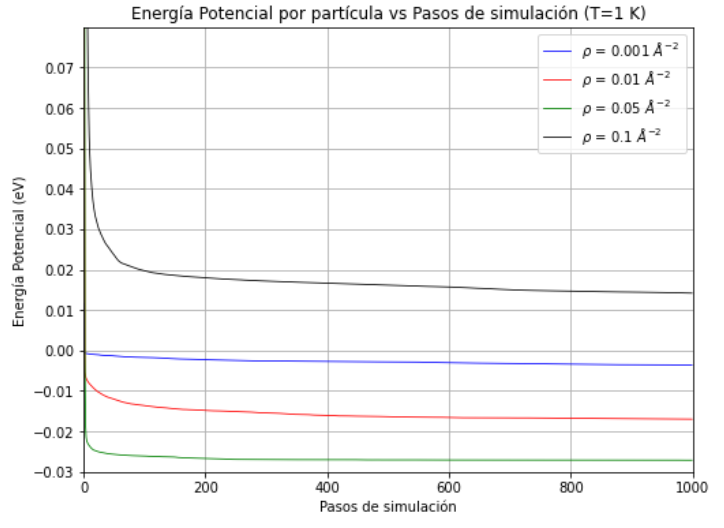
\includegraphics[width=1\textwidth]{grafico_3x22_termalizacion.png}
		\caption{\footnotesize Evolución de la energía potencial a través de la simulación para T=1 K, para todas los valores densidad.}
		\label{fig:termal}
	\end{minipage}%	
\end{figure}


\section{Conclusiones}

Las simulaciones de sistemas de partículas interactuando mediante el potencial de Lennard-Jones muestran una gran variedad de comportamientos y transiciones de fase en función de la densidad y la temperatura. 

\vspace{\baselineskip}

A bajas densidades (ρ=0.001 Å⁻²), el sistema exhibe características de un estado gaseoso, con partículas agrupándose preferentemente a distancias que corresponden al mínimo del potencial (r ≈ 3.8 Å). Estas agrupaciones forman estructuras básicas como dímeros, triángulos equiláteros y, ocasionalmente, romboidales.

\vspace{\baselineskip}

Al aumentar la densidad (ρ=0.01 Å⁻²), se observa una transición hacia un estado líquido, caracterizado por la aparición de picos adicionales en la función de distribución radial (RDF), indicativos de estructuras más complejas. La elevación de la temperatura en este régimen resulta en un ensanchamiento de los picos de la RDF, reflejando una mayor agitación térmica, aunque sin cambiar fundamentalmente el estado de agregación.

\vspace{\baselineskip}

Para densidades aún mayores (ρ=0.05 Å⁻²), el sistema transita a un estado sólido, evidenciado por una RDF con numerosos picos bien definidos, característicos de un orden de largo alcance. Sin embargo, el aumento de temperatura en este régimen puede inducir una fusión, desestabilizando las estructuras ordenadas y retornando el sistema a un estado líquido.

\vspace{\baselineskip}



A altas densidades  (\(\rho = 0.1 \, \text{Å}^{-2}\)) se ha encontrado un solapamiento aparente  entre partículas, donde manifestado por la obtención de mínimos de energía potencial a distancias menores que el mínimo característico del potencial de Lennard-Jones de \(3.81 \, \text{Å}\). En el análisis realizado, se sugiere que las fluctuaciones térmicas, en combinación con el potencial de Lennard-Jones, pueden inducir la aparición de nuevos mínimos energéticos a distancias inferiores.

\vspace{\baselineskip}

La dinámica de ordenamiento del sistema varía de manera compleja con la temperatura. A temperaturas moderadas, el proceso de ordenamiento se acelera, permitiendo que las partículas superen barreras energéticas locales y formen estructuras más organizadas. Sin embargo, a temperaturas muy elevadas, la energía cinética excesiva inhibe la formación de estructuras estables, manteniendo al sistema en un estado predominantemente desordenado


\vspace{\baselineskip}
En relación al proceso de termalización se ha  concluido que éste fue suficientemente largo para alcanzar el equilibrio a T=1K para todas las densidades estudiadas, y no sería necesario realizar más pasos de simulación para obtener resultados confiables del estado de equilibrio del sistema.


\vspace{\baselineskip}

Todas estas observaciones destacan la complejidad  de los sistemas regidos por el potencial de Lennard-Jones y su capacidad para modelar una amplia gama de fenómenos, desde la formación de estructuras básicas en gases diluidos hasta las transiciones de fase en sólidos y líquidos. 

\vspace{\baselineskip}


Para futuras trabajos cabría investigar como  casan estos resultado con los obtenidos en sistemas tridimensionales o  como podrían modificarse estos comportamientos en presencia de interacciones más complejas o campos externos.


\begin{thebibliography}{99}
	
\bibitem{Jones1924}
Jones, J. E. (1924). On the Determination of Molecular Fields. Proceedings of the Royal Society of London. Series A, Containing Papers of a Mathematical and Physical Character, 106(738), 463-477


\bibitem{metropolis1953}
Metropolis, N et al. (1953). Equation of State Calculations by Fast Computing Machines. The Journal of Chemical Physics, 21(6), 1087-1092.

\bibitem{Hastings1970}
Hastings, W. K. (1970). Monte Carlo Sampling Methods Using Markov Chains and Their Applications. Biometrika, 57(1), 97-109.

\bibitem{Frenkel2001}
Frenkel, D., Smit, B. (2001). Understanding Molecular Simulation: From Algorithms to Applications. Academic Press.

\bibitem{rf2022}
UNEDSoftMatter. RandomPhase. GitHub, 2022, \url{https://github.com/UNEDSoftMatter/RandomPhase}.




\end{thebibliography}
\newpage


% Cuarto artículo
\titleformat{\chapter}[display]
{\normalfont\bfseries}{}{0pt}{\LARGE}

\chapter{Análisis de curvas características de una célula solar.}
\begin{abstract}
	\vspace{\baselineskip}
	\footnotesize
	En este trabajo se analiza la respuesta de una termopila y un panel solar solar bajo distintas condiciones, incluyendo variaciones en la intensidad de luz, temperatura y distancia al foco de luz. En una serie de experimentos se han determinado las curvas intensidad-voltaje (I-V) en diferentes condiciones. además de como estos factores afectan al comportamiento de las células solares.
	
\end{abstract}
\section{Introducción}
% ***************************************

\vspace{\baselineskip}

Las células solares de silicio, convierten la luz solar en electricidad mediante el efecto fotoeléctrico. La caracterización de estas células  permiten entender y optimizar su rendimiento bajo diferentes condiciones operativas.

\vspace{\baselineskip}

Las curvas características corriente-voltaje $\text{I-V}$ de células solares de silicio bajo diferentes intensidades de luz y temperaturas permitan caracterizar el funcionamiento de las mismas y proporcionan información detallada sobre parámetros importantes como la corriente de cortocircuito $I_{SC}$, el voltaje de circuito abierto $V_{OC}$, y la potencia máxima ($P_{max}$) entre otros. Esto parámetros son relevantes para el análisis y la mejora del rendimiento de las células solares. Además, también se ha examinado la relación entre la intensidad de luz y la distancia a la fuente luminosa con el fin  de proporcionar una base para comprender la distribución de luz sobre las células solares en condiciones experimentales.

\vspace{\baselineskip}

En este trabajo se expone los resultados de varios experimentos llevados a cabo en laboratorio para determinar la respuestas de las células solares en varias condiciones específicas. 



\section{Fundamento teórico}
% ***************************************

Las termopilas y los paneles solares son dispositivos electrónicos capaces de generar una diferencia de potencial cuando la luz incide en ellos dentro de ciertos rangos de longitud de onda. Mientras que en los paneles solares, las células fotovoltaicas son sensibles a la luz, en una termopila, la sensibilidad principal es hacia la radiación infrarroja. Esta radiación infrarroja induce una diferencia de temperatura en los termopares de la termopila, lo que resulta en la generación de una diferencia de potencial a través del efecto Seebeck​​ [\cite{Goupil}].

\vspace{\baselineskip}

Las termopilas pueden emplearse para medir cambios en la intensidad de la luz basándose en el principio de que la cantidad de radiación infrarroja recibida varía con la distancia de la fuente de luz. Al posicionarse a diferentes distancias de una fuente de luz, las termopilas detectan variaciones en la radiación infrarroja, que se traducen en diferencias de temperatura en sus termopares. Estas diferencias de temperatura generan una diferencia de potencial a través del efecto Seebeck, que puede medirse y relacionarse con la intensidad de la luz incidente.

\vspace{\baselineskip}

En los paneles solares, la conversión de energía solar en electricidad se basa en el efecto fotoeléctrico. Este efecto se produce cuando los fotones que inciden sobre el material semiconductor provocan la formación de pares electrón-hueco. La generación de una corriente eléctrica se efectúa gracias a la existencia de una unión $pn$, que crea un campo eléctrico interno. Este campo dirige a los electrones hacia la zona $n$ y a los huecos hacia la zona $p$, impidiendo que se recombinen y facilitando así la creación de corriente eléctrica. La diferencia de potencial $V_0$ entre las áreas $p$ y $n$ es clave para determinar la eficiencia de la célula solar, la cual actúa semejantemente a un diodo en su funcionamiento.

\vspace{\baselineskip}

 


\vspace{\baselineskip}


El estudio de las curvas características corriente-voltaje \(I-V\) es fundamental para entender el comportamiento eléctrico de las células solares en variadas condiciones ambientales. De acuerdo con el modelo de Shockley para diodos \cite{boylestad_nashelsky}, la corriente a través del diodo \(I_D\) se puede expresar mediante la siguiente ecuación:
				
\vspace{\baselineskip}
\begin{equation}\label{eq:Id_shockley}
	I_D = I_0 \left( e^{\textstyle \frac{qV}{m k T}} - 1 \right)
\end{equation}
				
\vspace{\baselineskip}
				
en esta ecuación, $I_0$ representa la corriente de saturación inversa, $q$ es la carga elemental del electrón, $V$ el voltaje aplicado al dispositivo, $k$ se refiere a la constante de Boltzmann, $T$ es la temperatura expresada en Kelvin, y $m$ es el factor de idealidad del diodo, que describe su desviación respecto a un diodo ideal. Se observa que la corriente de saturación inversa incrementa con la temperatura y se puede calcular usando la expresión:
				
\begin{equation}
	I_0 = q A \left( \sqrt{\frac{D_p}{\tau_p}} \frac{n_i^2}{N_D} + \sqrt{\frac{D_n}{\tau_n}} \frac{n_i^2}{N_A} \right)
\end{equation}

\vspace{\baselineskip}
				
Aquí, $A$ denota el área de la sección transversal del diodo, $D_{p}$ y $D_{n}$ son los coeficientes de difusión para huecos y electrones respectivamente, $N_{D}$ y $N_{A}$ son las densidades de dadores y aceptores en las regiones $N$y $P$, respectivamente, $n_{i}$ es la concentración intrínseca de portadores de carga en el semiconductor, y $\tau_{p}$ y $\tau_{n}$ son los tiempos de vida de los portadores de huecos y electrones, respectivamente.



\vspace{\baselineskip}

Desde las curvas I-V, se pueden determinar la corriente de cortocircuito $I_{SC}$ y el voltaje de circuito abierto $V_{OC}$, siendo $I_{SC}$ el indicador de la máxima corriente producida bajo iluminación y $V_{OC}$ el máximo voltaje generado en ausencia de carga. Estos parámetros son esenciales para evaluar la eficiencia de las células solares, la cual también depende del factor de forma $FF$ y la resistencia interna $R_i$. El $FF$ se define como:

\begin{equation}\label{eq:factorforma}
FF = \frac{P_{max}}{V_{OC} I_{SC}}
\end{equation}

\vspace{\baselineskip}

donde $P_{max}$ es la potencia máxima extraíble de la célula solar. 

\vspace{\baselineskip}

La resistencia de carga o característica  $R_{ch}$, es la correspondiente al punto de máxima potencia que, concretamente en ese punto coincide con la resistencia interna $R_i$.


\vspace{\baselineskip}


\begin{equation}\label{eq:Ri}
R_{ch} = R_{i, Pmax} = \frac{V_{Pmax}}{I_{Pmax}}
\end{equation}

\vspace{\baselineskip}

Finalmente el rendimiento $\eta$ de una célula solar, puede ser expresada según \ref{eq:rendimiento}, donde  $P_L$ es la potencia de la luz incidente dada por el producto de la irradiancia y la superficie efectiva $S_e$ del panel solar.

\begin{equation}\label{eq:rendimiento}
\eta= \frac{P_{\max}}{P_{L}}= \frac{P_{\max}}{J\cdot S_e}
\end{equation}
		
\vspace{\baselineskip}
		
El rendimiento es también influenciado por el espectro y la intensidad de la luz solar que incide sobre ella, así como por su temperatura operativa. De ahí la importancia de estandarizar las condiciones bajo las cuales se evalúa la eficiencia para permitir comparaciones fiables entre distintos dispositivos.

\vspace{\baselineskip}

Por otro lado, la temperatura, de acuerdo a \ref{eq:Id_shockley}, influye en el comportamiento de una batería solar. De hecho si se disponen las curvas características de la batería a dos temperaturas diferentes es posible calcular el coeficiente de temperatura del voltaje de circuito abierto $\beta$ [\ref{eq:coef_temperatura}], que proporciona la disminución de voltaje generado por el panel al aumentar la temperatura 1 K, cuando éste está sin carga alguna (circuito abierto).

\begin{equation}\label{eq:coef_temperatura}
	\beta= \frac{V_{oc}(T) - V_{oc}(T_{ref}) }{T - T_{ref}}
\end{equation}


donde:

\begin{itemize}
	\setlength\itemsep{0.05em}
	\item $V_{oc}(T)$ es el voltaje de circuito abierto a la temperatura $T$,
	\item $V_{oc}(T_{ref})$ es el voltaje de circuito abierto a la temperatura de referencia $T_{ref}$.
	\item $\beta$ es el coeficiente de temperatura del voltaje de circuito abierto expresado en (V/°C) o (mV/K) dependiendo del contexto.
	\item $T$ es la temperatura del panel solar en grados Celsius o Kelvin,
	\item $T_{ref}$ es la temperatura de referencia, por lo general 25°C o 298 K).
\end{itemize}


\section{Experimentos y resultados}

A continuación se pasará a describir los experimentos llevados a cabo junto con los resultados que se han derivado de la toma de datos correspondiente.

\vspace{\baselineskip}

No obstante, antes de entrar en detalle es necesario explicar el criterio aplicado en la propagación de errores. Ésta se ha llevado siguiendo dos criterios. En primer lugar en el caso de expresiones que son combinación lineal de variables, se ha llevado a cabo una propagación lineal [\ref{eq:prop_lin}]. 

\vspace{\baselineskip}

\begin{equation}\label{eq:prop_lin}
	{\Delta f} = \left|\mathbf{\nabla}f\right|\cdot\mathbf{\Delta x} =  \sum_{i=1}^{n}\left|\frac{\partial f}{\partial x_i}\right|\Delta x_i
\end{equation}

\vspace{\baselineskip}

En caso de expresiones no lineales, se ha optado por hacer una propagación de errores basada en el método de Montecarlo [\cite{Anderson_montecarlo}], [\cite{montacarlo_python}], generando 1000 muestras de las variables implicadas de acuerdo a una distribución normal centrada en la medida y tomando la incertidumbre como desviación típica.  Para cada muestra se ha calculado el valor de la función correspondiente siendo la estimación final el valor medio de la distribución obtenida y su incertidumbre la desviación típica. Matemáticamente, el proceso se puede resumir como:

\begin{enumerate}
\item Generar muestras: \((x_{1j}, x_{2j}, \ldots, x_{nj})\) para \(j = 1, 2, \ldots, N\)
\item Calcular: \(f_j = f(x_{1j}, x_{2j}, \ldots, x_{nj})\)
\item Analizar: \(\mu_f = \text{media}(f_j)\), \(\sigma_f = \text{desviación estándar}(f_j)\)
\end{enumerate}

\vspace{\baselineskip}

Dicho lo anterior, el primero de los experimentos que se ha llevado a cabo tuvo por objeto analizar el decaimiento de la irradiancia $J$ con la distancia al incidir esta sobre una termopila de 22.69 $\mu V/Wm^{-2}$ de sensibilidad. La expresión para el cálculo de $J$ viene dada por [\ref{eq:irradiancia}].

\vspace{\baselineskip}

\begin{equation}\label{eq:irradiancia}
	J = \frac{V_{th}}{S}
\end{equation}

\vspace{\baselineskip}

donde $V_{th}$ es el voltaje medido por la termopila y $S$ la sensibilidad de la misma. 

\vspace{\baselineskip}

En tal experimento se han realizado medidas del voltaje generado en la termopila situando ésta a diferentes distancias de la lámpara (tabla \ref{tab:medidas_voltajes}). Esto ha permitido determinar el valor de la irradiancia $J$ y ver su evolución con la distancia según se muestra en la figura  \ref{fig:irradiancia_distancia}.

\vspace{\baselineskip}

\begin{table}[H]
	\centering
	$\Delta V=$ 0.1 mV; $\Delta d=$0.2 cm; $S =$ 22.69\pm 0.01$\, \mu V/Wm^{-2}$ \\ 
	\begin{threeparttable}
		\begin{tabular}{c|c|c}
			\toprule
			\toprule
			$\qquad d\,(\text{cm})\qquad$ & $\qquad V_{th}\,(\text{mV})\qquad$ & $\qquad J\,(\text{W/m}^2)\qquad$    \\
			\midrule		
			63 & 13.87 & 611$\pm$4  \\
			70 & 11.30 & 498$\pm$4  \\
			80 &  8.12 & 358$\pm$4  \\
			90 &  6.28 & 277$\pm$4  \\
			100 & 4.93 & 217$\pm$4  \\
			110 & 4.00 & 176$\pm$4  \\
			120 & 3.35 & 148$\pm$4  \\
			147* & 0.00* & 0.00*   \\
			\bottomrule
			\bottomrule
		\end{tabular}
		\caption{Medidas de voltaje para cada distancia. Valores de la irradiancia $J$ calculada.}
		\label{tab:medidas_voltajes}
	\end{threeparttable}
\end{table}

\vspace{\baselineskip}

También se puede observar en dicha tabla, que la medida de voltaje para una distancia de 147 cm no fue correcta y fue descartada en el gráfico log-log (figura \ref{fig:irradiancia_distancia}b). 

\vspace{\baselineskip}

El ajuste lineal por mínimos cuadrados, (figura \ref{fig:irradiancia_distancia}b),  describe claramente un patrón lineal entre los logaritmos de la distancia y la irradiancia. Este ajuste se ha llevado a cabo mediante el método de Montecarlo, generando 10000 muestras y sus respectivas regresiones lo que ha permitido determinar la incertidumbre en la pendiente y en el término independiente, las incertidumbres de la variables de partida se indican en la tabla \ref{tab:medidas_voltajes}.



\begin{equation}\label{eq:ajuste_logJ}
		log_{10}(J) = (-2.24\pm 0.03)\cdot log_{10}\,(d) + 6.81\pm 0.06 = log_{10}(\frac{10^{6.81\pm0.06}}{d^{2.24\pm 0.03}} ) \rightarrow \boxed{J = \frac{10^{6.81\pm 0.06}}{d^{2.24\pm 0.03}}}
\end{equation}

\vspace{\baselineskip}

El valor de la pendiente de la recta obtenida $-2.24\pm 0.04$, indica que la intensidad decae con la distancia pero sin llegar cumplirse $J \propto \frac{1}{d^2}$.


\begin{figure}[H]
	\centering
	\begin{subfigure}{0.42\textwidth}
		\centering
		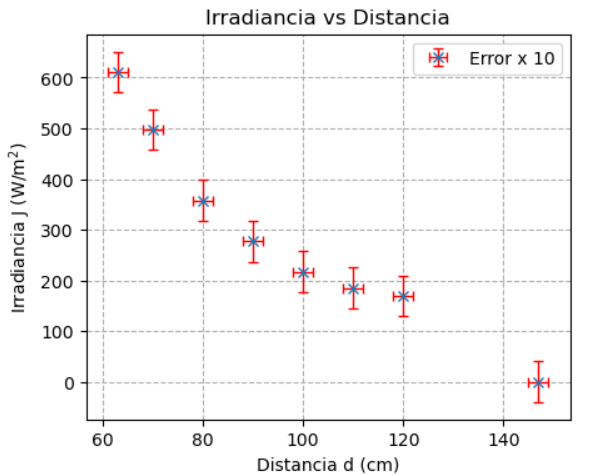
\includegraphics[width=\textwidth]{grafico01_irradiancia_vs_distancia.png}
		\caption{}\label{fig:a}
	\end{subfigure}\hspace{1cm} % Ajusta el espacio horizontal según sea necesario
	\begin{subfigure}{0.51\textwidth}
		\centering
		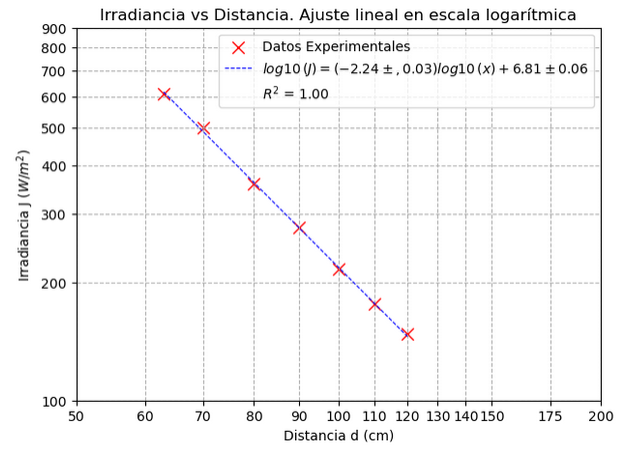
\includegraphics[width=\textwidth]{grafico02_ajuste_loglog_irradiancia_vs_distancia.png}
		\caption{}\label{fig:b}
	\end{subfigure}
	\caption{Representación grafíca Irradiancia vs Distancia. (a) Escala normal con barras de error. (b) Ajuste lineal en gráfico $log_{10}-log_{10}$.}
	\label{fig:irradiancia_distancia}
\end{figure}

\vspace{\baselineskip}

En el siguiente experimento se ha obtenido la curva característica $\text{I-V}$ de una celda solar a 70, 110 y 150 cm de distancia de una lámpara. En la gráfica [\ref{fig:curvas_caracteristicas}], se muestran las curvas obtenidas con los puntos de máxima potencia respectivos en cada una de ellas de acuerdo a los puntos medidos. La obtención de estos puntos máximos permite hacer una estimación de algunos de los parámetros vistos en la sección de fundamento teórico tal y como se muestra en la tabla [\ref{tab:iv_parametros}]

\vspace{\baselineskip}

\begin{figure}[H]
	\centering
	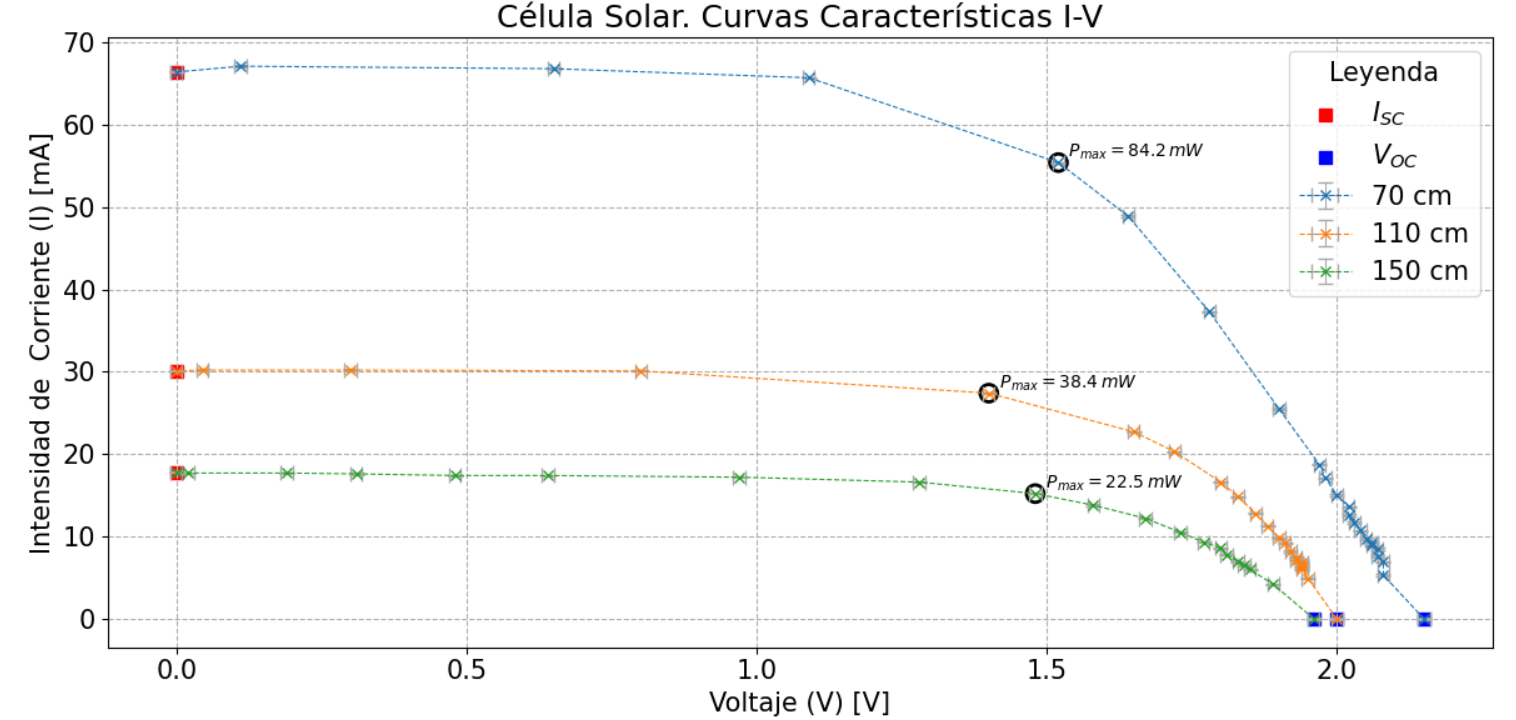
\includegraphics[width=0.9\textwidth]{grafico03_curvas_caracteristicas_celula_solar}
	\caption{Curvas características de la célula solar para diferente distancias al foco de luz.}
	\label{fig:curvas_caracteristicas}
\end{figure}



\begin{table}[H]
	\centering
	\scalebox{0.9}{
	\begin{tabular}{ccccccccc}
		\hline
		$d \text{(cm)}$ & $I_{Pmax} \text{(mA)}$ &  $V_{Pmax}\text{(V)}$ & $I_{SC}\text{(mA)}$ & $V_{OC}\text{(V)}$ &  $P_{\text{max}}\text{(mW)}$ & $R_{i,Pmax} \text{(\Omega)}$  & $FF$ & $\eta$ ($\%$) \\
		\hline
		70  & 55.4$\pm$ 0.1 & 1.52$\pm$ 0.01 & 66.4$\pm$ 0.1 & 2.15$\pm$ 0.01 &  84.2$\pm$ 0.6 & 27.4$\pm$0.2 & 0.59$\pm$0.01   & 3.4$\pm$0.0 \\
		110 & 27.4$\pm$ 0.1 & 1.40$\pm$ 0.01 & 30.1$\pm$ 0.1 & 2.00$\pm$ 0.01 &  38.4$\pm$ 0.3 & 51.1$\pm$0.4   & 0.64$\pm$0.01 & 4.4$\pm$0.1  \\
		150 & 15.2$\pm$ 0.1 & 1.48$\pm$ 0.01 & 17.8$\pm$ 0.1 & 1.96$\pm$ 0.01 &  22.5$\pm$ 0.2 & 97.4$\pm$0.9 & 0.65$\pm$0.01   & 5.4$\pm$1.4 \\
		\hline
	\end{tabular}
	}
	\caption{Datos de caracterización de las curvar I-V. Área del panel solar A = 50 cm$^2$.}
	\label{tab:iv_parametros}
\end{table}


\vspace{\baselineskip}

Dado que las expresiones $P_{max}$,  factor de forma $FF$ y el rendimiento $\eta$ y la resistencia característica $R_{ch}$ son no lineales  se ha empleado el método de Montecarlo para estimar la incertidumbre en \(R_i\),  según se comentó al principio de esta sección.


\vspace{\baselineskip}

 Para el cálculo del rendimiento se han tomado los valores calculados de irradiancia de la tabla \ref{tab:medidas_voltajes}. Dado que para el  valor $d=150$ cm no se dispone de medida de irradiancia, se ha empleado la expresión del ajuste [\ref{eq:ajuste_logJ}], arrojando un valor $J_{150} =  88\pm$18 W/m$^2$.

\vspace{\baselineskip}

En el tercer experimento, se han tomado medidas $I_{SC}$ y $V_{OC}$ para diferentes distancias y, además, se ha obtenido el valor del factor de proporcionalidad $a = 0.127\pm0.004$ mA/Wm$^{-2}$, o lo que es lo mismo $a=1.27\pm0.04 \cdot 10^{-4}$ A/Wm$^{-2}$, entre la corriente de cortocircuito y la irradiancia (ver Figura \ref{fig:Voc_Isc_J}). Dado que la irradiancia en el experimento 1 no se determinó para las distancias de 130, 140 y 150 cm, se ha empleado la expresión (\ref{eq:ajuste_logJ}) para su cálculo.


\vspace{\baselineskip}

\begin{figure}[H]
	\centering
	\begin{subfigure}{0.46\textwidth}
		\centering
		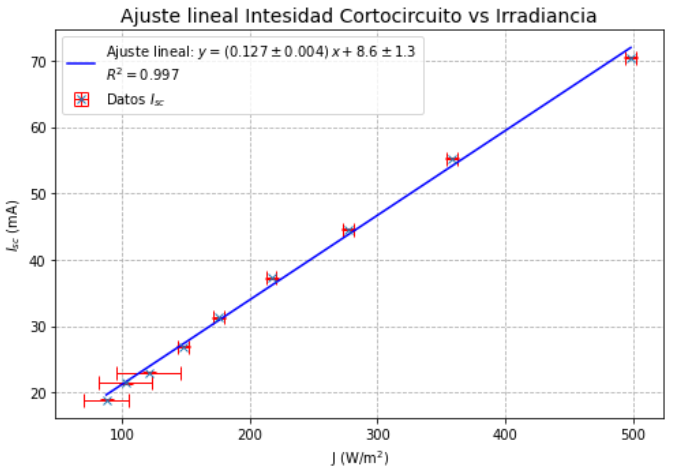
\includegraphics[width=\textwidth]{grafico04_ajuste_Isc_irradiancia.png}
		\caption{}\label{fig:a}
	\end{subfigure}\hspace{1cm} % Ajusta el espacio horizontal según sea necesario
	\begin{subfigure}{0.46\textwidth}
		\centering
		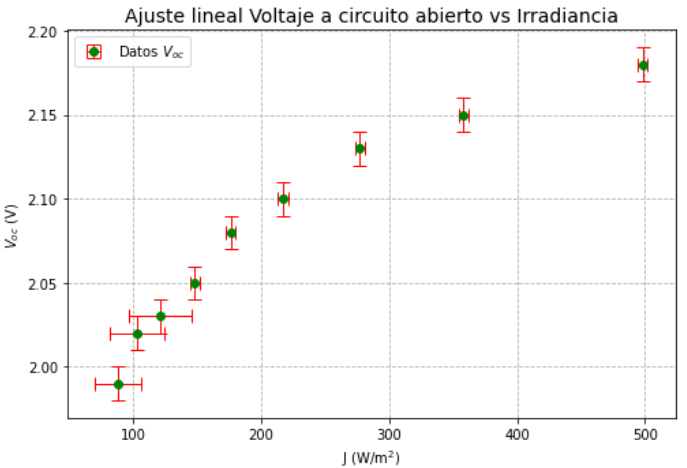
\includegraphics[width=\textwidth]{grafico05_puntos_Voc_irradiancia.png}
		\caption{}\label{fig:b}
	\end{subfigure}
	\caption{(a) Variación de la intensidad de cortocircuito $I_{sc}$ con la irradiancia J y ajuste lineal. (b) Variación de la diferencia potencial a circuito abierto $V_{oc}$ con la irradiancia J.}
	\label{fig:Voc_Isc_J}
\end{figure}

\vspace{\baselineskip}

La temperatura es también un factor en cuenta en el comportamiento de una celda solar expresiones de acuerdo al modelo de Shockley [\ref{eq:Id_shockley}]. Para analizar esta cuestión, se llevó  a cabo un cuarto experimento en donde se han determinados las curvas características del panel solar tanto a temperatura ambiente de 24.5 °C como a  a 72 °C, ambas a una distancia de 110 cm del foco de luz. [figura \ref{fig:I_V_temperatura}].  Esto ha permitido hacer una estimación del coeficiente de temperatura a en relación al voltaje a circuito abierto \ref{eq:coef_temperatura}, tomando como temperatura de referencia 24.5 °C. El valor obtenido es:

\vspace{\baselineskip}

\begin{equation}\label{eq:beta_VT}
	\beta= \frac{\Delta V_{OC}}{\Delta T} = \frac{1990 \text{ mV} - 2010 \text{ mV} }{345 \text{ K}  - 297.5 \text{ K} } = -0.4\pm 0.3 \text{ mV/K} 
\end{equation}

\vspace{\baselineskip}

Como se observa es un medida muy poco precisa. Este y otros aspectos relacionados se tratarán en la sección de discusión de los resultados.


\vspace{\baselineskip}

La propagación del error se ha llevado a cabo por el metodo de Montecarlo con unas incertidumbres $\Delta T$=0.1 K para la temperatura y $\Delta V$=0.01 V para el voltaje. La medida de $V_{OC}$ para una distancia de 110 cm ya se ha medido previamente en dos ocasiones en los experimentos 2 y 3. Para este experimento se hizo una medida adicional que arrojó un valor de 2.01 V que es el que se ha empleado en la expresión anterior. 

\vspace{\baselineskip}


\begin{figure}[H]
	\centering
	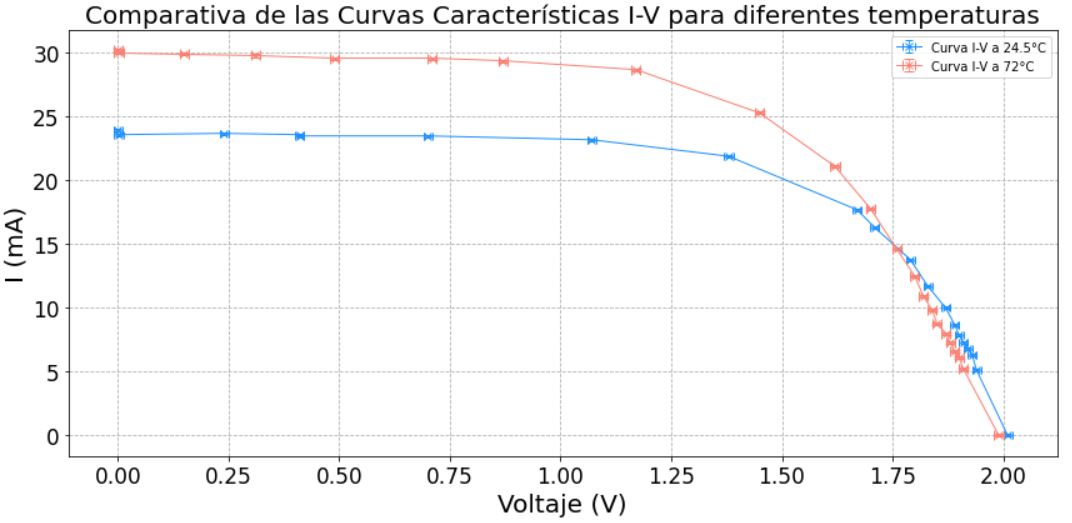
\includegraphics[width=0.75\textwidth]{grafico06_I_V_temperatura.png}
	\caption{Comparativa de curvas características a una distancia de 110 cm del foco de luz para temperaturas de 24.5 °C y a 72 °C.}
	\label{fig:I_V_temperatura}
\end{figure}


\vspace{\baselineskip}


Finalmente en quinto y último experimento, se ha calculado la irradiancia y la curva característica del panel en el exterior usando el sol como fuente de luz \ref{fig:I_V_luz_solar}. Así mismo se han calculado los parámetros de caracterización correspondientes \ref{tab:iv_parametros_sol}.


\begin{figure}[H]
	\centering
	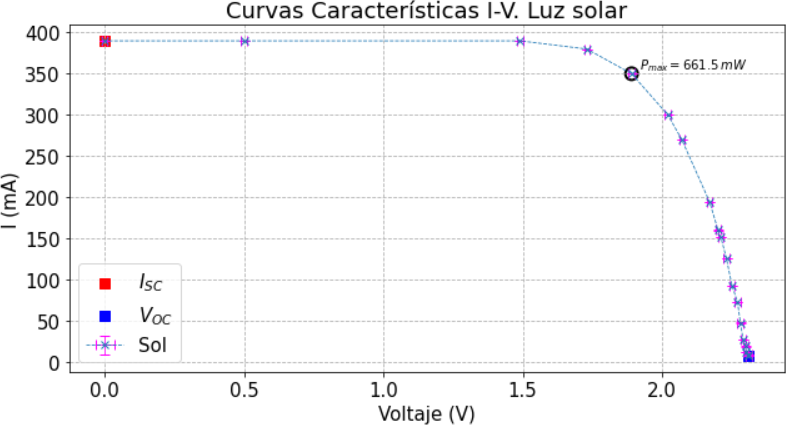
\includegraphics[width=0.65\textwidth]{grafico07_I_V_luz_solar.png}
	\caption{Curva Característica I-V de la batería solar bajo luz solar exterior.}
	\label{fig:I_V_luz_solar}
\end{figure}

\begin{table}[H]
	\centering
	$S =$ 22.69\pm 0.01$\, \mu V/Wm^{-2}$; $V_{th}$ = 25,9$\pm$0.1 mV \\ 
	\scalebox{0.8}{
		\begin{tabular}{ccccccccc}
			\hline
			J \text{(W/m}$^2$) & $I_{Pmax} \text{(mA)}$ &  $V_{Pmax}\text{(V)}$ & $I_{SC}\text{(mA)}$ & $V_{OC}\text{(V)}$ &  $P_{\text{max}}\text{(mW)}$ & $R_{i,Pmax} \text{(\Omega)}$  & $FF$ & $\eta$ ($\%$) \\
			\hline
			1008$\pm$ 4 & 350$\pm$ 0.1 & 1.89$\pm$ 0.01 & 390$\pm$ 0.1 & 2.31$\pm$ 0.01 &  662$\pm$ 3 & 5.40$\pm$0.02 & 0.734\pm$0.005$   & 13.1\pm$0.1$ \\
			\hline
		\end{tabular}
	}
	\caption{Parámetros de caracterización de la curvas I-V del panel solar bajo luz solar exterior. Área del panel solar A = 50 cm$^2$.}
	\label{tab:iv_parametros_sol}
\end{table}


De nuevo en este caso la propagación del error se ha llevado a cabo por el método de Montecarlo.

\section{Discusión}




La relación entre la irradiancia y la distancia a la fuente de luz, obtenida en el primer experimento, ha mostrado una tendencia decreciente, la cual, en principio, se alinea con el modelo teórico de disminución inversamente proporcional al cuadrado de la distancia, característico de fuentes puntuales de luz o que, de acuerdo a la escala observada, pueden considerarse como puntuales. Sin embargo, la pendiente obtenida en el ajuste lineal de $-2.24 \pm 0.04$ [figura \ref{fig:irradiancia_distancia}],  indica una desviación de este modelo. Esta desviación podría ser atribuible a varios factores físicos y experimentales. Aspectos como la reflexión y refracción de la luz ambiental en el entorno o la respuesta no uniforme de la termopila a distintas longitudes de onda, pueden alterar este comportamiento. La geometría de la lámpara halógena como fuente de luz también debe ser considerada dado que, a diferencia de una fuente puntual, tiene una extensión física que puede contribuir a la divergencia del modelo de fuente puntual a distancias cortas [\cite{Shibuya_notsquared}]. Dada la naturaleza del experimento, el comportamiento no ideal observado sugiere la necesidad de un modelo más complejo que pueda abarcar estas no linealidades o efectos de borde. Como en cualquier montaje experimental, cuestiones como la precisión en la medición de las distancias o la alineación de la termopila con respecto al centro de la lámpara también han podido tener su influencia, aunque el claro ajuste obtenido sugiere que este aspecto ha tenido poco peso.




\vspace{\baselineskip}	

Los datos obtenidos para el trazado de las curvas características I-V  de la célula solar a diferentes distancias de una fuente de luz [Figura ]\ref{fig:curvas_caracteristicas}b] muestran una disminución de la corriente de cortocircuito $I_{SC}$ y la tensión de circuito abierto $V_{OC}$ a medida que la distancia a la fuente de luz aumenta, lo cual se atribuye a la menor irradiancia recibida por la célula. Esta disminución en $I_{SC}$ y $V_{OC}$ lleva, a su vez, a una reducción en la potencia máxima $P_{max}$ obtenida de la célula. Por otro lado, cabría esperar una cierta alineación de los puntos de máxima potencia en las curvas I-V, la cual, para los tres puntos disponibles, no se observa de una forma clara. Esto sugiere la influencia de otros factores en las mediciones o bien una resolución insuficiente en el muestreo de datos. En este sentido, disponer tanto curvas I-V adicionales como una mayor densidad de puntos alrededor del punto de máxima potencia podría proporcionar una representación más precisa de la curva, facilitando una mejor comprensión de la respuesta de la célula y una estimación más exacta de sus parámetros óptimos de operación.  


\vspace{\baselineskip}	

En lo referente a la resistencia interna a máxima a potencia máxima, se observa que aumenta con la distancia, reflejando una disminución en la potencia generada al alejarnos cada vez mas del foco más que cambios en las propiedades intrínsecas de la célula solar. 



\vspace{\baselineskip}	

Por otro lado, el factor de forma $FF$ compara el punto de máxima potencia en la curva I-V con la disponibilidad máxima teórica de potencia dada por el producto $I_{SC}\cdot V_{OC}$, asumiendo estas últimas como una características ideales de operación. Los valores obtenidos para $FF$ en la tabla [\ref{tab:iv_parametros}] sugieren un aumento del mismo al aumentar la distancia, pero dado que solo se disponen de tres puntos,  no se puede descartar que el valor sea constante o en todo caso establecer una patrón claro de variación. De hecho, si los datos se interpretan como $FF$ constante, esto sugeriría que, en el rango de distancias del experimento, habría un mayor peso en las características internas de la celda que de las condiciones externas de operación. Al contrario  ocurriría si se interpreta que el $FF$ aumenta con la distancia. Entre estas dos interpretaciones extremas cabe considerar la influencia de tantos factores internos de la celda como externos, pero para llegar a una conclusión más sólida sería necesario disponer de más valores de $FF$ a otras distancias. En este último escenario tendrían cabida modelos en donde $FF$ podría llegar a un máximo que podría ser asintótico o bien alcanzarse para cierta distancia dada una cierta irradiancia. El rango de valores del factor de forma obtenido para en el experimento es de 0.59-0.65 que es algo inferior al rango habitual para celdas de silicio que se situa en el rango 0.70-0.85 [\cite{solar_eff}], si bien esta comparación se da como orientativa ya que no son comparables las condiciones de experimentales en ambos casos.    

\newpage

De acuerdo a los tres puntos de rendimiento obtenidos para la celda, éstos tienen comportamiento similar al del factor de forma y la discusión anterior es válida igualmente dada la interrelación entre ambos parámetros de acuerdo a las expresiones [\ref{eq:factorforma}] y [\ref{eq:rendimiento}]. De forma orientativa el rendimiento de las celdas solares de silicio se sitúa actualmente por encima del 15\% [\cite{solar_eff}].

\vspace{\baselineskip}	

En relación al tercer experimento, donde se analiza la variación de la corriente de cortocircuito $I_{SC}$ y la tensión de circuito abierto $V_{OC}$ en función de la irradiancia $J$, los resultados presentados en la figura [\ref{fig:Voc_Isc_J}a] reflejan  claramente una correlación lineal entre $I_{SC}$ y $J$ siendo la estimación obtenida para el factor de proporcionalidad $a=(1.27\pm0.04$)$\cdot10^{-4}$ A/Wm$^{-2}$.  Por otro lado, el voltaje a circuito abierto, $V_{oc}$, no muestra una dependencia lineal tan clara como la $I_{sc}$, tal y como se observa en la dispersión de los puntos en la figura [\ref{fig:Voc_Isc_J}b]. Aunque la tendencia general sugiere un aumento de $V_{oc}$ con la irradiancia, tal crecimiento se atenúa progresivamente, siendo el patrón de los datos compatible con una convergencia asintótica a cierto valor del voltaje a circuito abierto.

\vspace{\baselineskip}	

La dependencia del comportamiento de las celdas solares respecto a la temperatura es otro aspecto relevante a estudiar. En este sentido en el cuarto experimento se trató de determinar el coeficiente de variación de voltaje en relación a la variación de temperatura \ref{eq:beta_VT}. El valor estimado para el coeficiente de temperatura $\beta$ de -0.4$\pm$ 0.3 mV/K indica una marcada incertidumbre. Además este valor difiere del valor aproximado dado por el fabricante del panel de -2 mV/K. Una de las causas de esta disparidad podría radicar en que las mediciones se han realizado solo para dos temperaturas, lo que deriva en una estimación demasiado superficial. Lo recomendable hubiera sido considerar curvas I-V para temperaturas adicionales, obteniendo así más puntos de datos y permitiendo un ajuste por regresión más preciso. Otro factor que podría haber influido en la toma de datos es la homogeneidad de la temperatura en el panel. El calentamiento del aire circundante al panel puede no haber sido homogéneo y haber creado gradientes de temperaturas que han podido distorsionar las medidas del voltaje e intensidad. Además, la convección y la conductividad térmica del aire circundante, junto con la inercia térmica del propio panel, pueden haber conducido a discrepancias entre la temperatura del aire y la del panel, lo cual es relevante para la correcta asignación de la temperatura al momento de las mediciones.

\vspace{\baselineskip}	

Dicho lo anterior, con las dos curvas I-V que se muestran en la figura [\ref{fig:I_V_temperatura}] se observa  un descenso de $V_{OC}$  y aumento de la intensidad de $I_{SC}$al aumentar la temperatura. La disminución $V_{OC}$ es atribuible a la reducción en la brecha de energía del material semiconductor con el aumento de la temperatura, lo que incrementa la generación de portadores de carga en el material y reduce la barrera de potencial que se puede establecer en la unión p-n del panel fotovoltaico. Consecuentemente, es necesario un menor voltaje para poner en movimiento los portadores de carga, resultando en una menor $V_{oc}$, lo que conlleva a su vez un aumento del flujo de electrones y por tanto de la intensidad.

\vspace{\baselineskip}	


En relación al quinto y último experimento, los resultados obtenidos muestran un buen rendimiento del panel solar bajo luz solar exterior, como se observa en la curva característica I-V y los parámetros de caracterización.  De acuerdo a la tabla \ref{tab:iv_parametros_sol}, la corriente de cortocircuito ($I_{SC}$) de 390 mA y el voltaje de circuito abierto $V_{OC}$) de 2.31 V son consistentes con las expectativas para un panel solar en estas condiciones, indicando una buena respuesta a la irradiancia. La potencia máxima de 662 mW demuestra la eficiencia del panel, mientras que la eficiencia del 13.1\% y el factor de forma de 0.734 reflejan una buena calidad de la curva I-V. Además, la baja resistencia interna en el punto de máxima potencia (5.40 $\Omega$) sugiere que las pérdidas internas son mínimas, contribuyendo positivamente a la eficiencia del panel. En conjunto, estos resultados evidencian un comportamiento nominal del panel solar cuando se expone a la luz solar directa [\cite{solar_eff}].

\vspace{\baselineskip}	

Por otro lado, el valor de $I_{sc}$ obtenido a partir del gráfico I-V es de 390$\pm$0.1 mA, que es claramente superior al valor máximo de  $I_{sc}$ obtenido en el experimento 3, que es de 70.5$\pm$0.1 mA. Esta diferencia de intensidad es debida a las diferencias en los espectros de las fuentes de luz y como se relacionan éstos con la sensibilidad espectral de la célula de solar. El espectro solar contiene menos energía en la parte del infrarrojo en comparación con una lámpara incandescente, como se puede observar en la gráfica \ref{fig:Respuesta_espectral}. Esto significa que la luz solar tiene una mayor proporción de fotones de alta energía en el rango visible y ultravioleta, los cuales son más efectivos para generar corriente en una célula solar de silicio. Además, la menor cantidad de energía infrarroja en el espectro solar implica que la célula solar se calienta menos, lo que ayuda a mantener su eficiencia en la conversión de luz a electricidad. Por el contrario, la lámpara incandescente emite más energía en el infrarrojo, lo que no solo es menos eficiente para generar corriente en la célula de silicio, sino que también causa más calentamiento, reduciendo así la eficiencia de la célula.
 
 \begin{figure}[H]
 	\centering
 	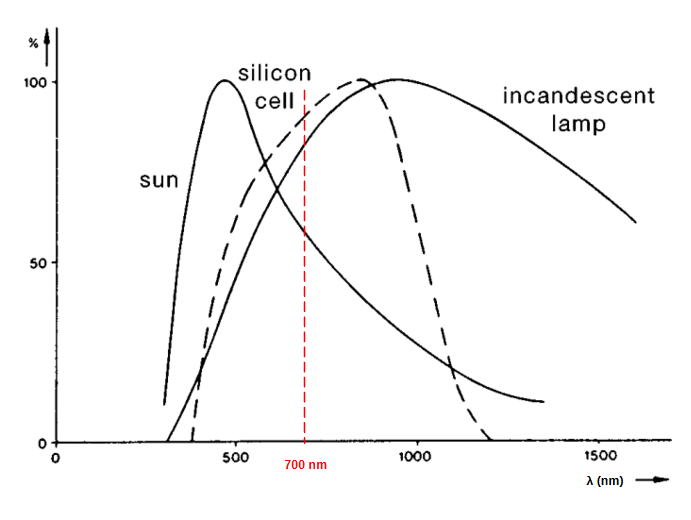
\includegraphics[width=0.6\textwidth]{grafico08_respuesta_espectral.png}
 	\caption{Espectro Solar (T aprox. 5800 K) y de una lámpara incandescente (T aprox. 2000 K) y la
 		sensibilidad espectral de una célula solar de silicio. La linea de 700 nm marca el comienzo de la transición rojo-infrarojo.}
 	\label{fig:Respuesta_espectral}
 \end{figure}

\section{Conclusiones}


Los experimentos realizados han permitido analizar el comportamiento de las células solares bajo diversas condiciones. Se observó que la relación entre irradiancia y distancia a la fuente de luz no sigue exactamente el modelo teórico de disminución inversamente proporcional al cuadrado de la distancia. Esto sugiere la necesidad de un modelo más complejo que considere factores como la reflexión, la refracción y la geometría de la lámpara.

\vspace{\baselineskip}	

Las mediciones de las curvas características I-V mostraron que tanto la corriente de cortocircuito como la tensión de circuito abierto disminuyen con la distancia a la fuente de luz, resultando en una reducción de la potencia máxima. No obstante, la falta de alineación clara en los puntos de máxima potencia indica la influencia de otros factores y la necesidad de una mayor densidad de datos para una evaluación más precisa. Además, se observó una relación lineal clara entre la corriente de cortocircuito y la irradiancia, mientras que la tensión de circuito abierto mostró una tendencia asintótica, sugiriendo que la respuesta de la célula solar a la irradiancia no es completamente lineal.

\vspace{\baselineskip}	

La variación del voltaje con la temperatura presentó alta incertidumbre, con discrepancias respecto a los valores teóricos proporcionados por el fabricante, subrayando la importancia de obtener más puntos de medición y un control de temperatura más preciso para mejorar la estimación del coeficiente de temperatura.

\vspace{\baselineskip}	

Por último, se demostró que la luz solar es más eficiente que la luz de una lámpara incandescente para las células solares de silicio, debido a una mayor proporción de fotones de alta energía y menor calentamiento. Esto resalta la relevancia del espectro de luz en la eficiencia de conversión de las células solares.

\vspace{\baselineskip}	

En conjunto, estos resultados proporcionan un conocimiento más detallado del funcionamiento de las células solares bajo diferentes condiciones de irradiancia, temperatura y espectro de luz, contribuyendo a una mejor comprensión de su comportamiento y rendimiento en aplicaciones prácticas.

\clearpage

\begin{thebibliography}{99}
	
	\bibitem{Goupil} Goupil, C, \textit{Continuum Theory and Modeling of Thermoelectric Elements}. Wiley-VCH. ISBN: 978-3-527-41337-9, 2016 
	
	\bibitem{boylestad_nashelsky} Boylestad R.L., L. Nashelsky, \textit{Electronic Devices and Circuit Theory}, Prentice Hall, 2014.
	
	\bibitem{solar_eff} Green, M., Dunlop, E., Hohl‐Ebinger, J., Yoshita, M., Kopidakis, N., Hao, X.,  \textit{Solar cell efficiency tables, version 57},  Progress in Photovoltaics: Research and Applications, 2020, \href{https://doi.org/10.1002/pip.3371}{doi:10.1002/pip.3371}
		
	\bibitem{Anderson_montecarlo} Anderson, G. M., \textit{Error propagation by the Monte Carlo method in geochemical calculations}, Geochimica et Cosmochimica Acta, 40(12), 1533-1538, 1976
	
	\bibitem{error_prop} Bevington, Philip R., y D. Keith Robinson. \textit{Data Reduction and Error Analysis for the Physical Sciences}. 3ra ed., McGraw-Hill, 2003.
	
	\bibitem{Shibuya_notsquared} Shibuya T., Kitaguchi K., Iwanaga T., \textit{The inverse square law in metrology considering a finite photosensitive area}., 52(3):407-412, 2020, \href{https://doi.org/10.1177/1477153519871324}{doi:10.1177/1477153519871324}.
	
	\bibitem{montacarlo_python} Santiago F., \textit{Python Code for Error Propagation Algorithms Using Monte Carlo Simulations and Other Methods} [Software], \url{https://github.com/fransantiago-lab/error_propagation}, 2024
	
	
	

	
	



	
\end{thebibliography}

    
   
\end{document}



